\documentclass[11pt]{article}

\usepackage[T1]{fontenc}
\usepackage[utf8]{inputenc}
\usepackage{charter}
\usepackage[scaled=0.9]{helvet}
\usepackage{courier}
\usepackage[margin=1in]{geometry}
\usepackage{microtype}
\usepackage{amsmath,amssymb}
\usepackage{booktabs}
\usepackage{tabularx}
\usepackage{longtable}
\usepackage{array}
\usepackage{enumitem}
\usepackage[dvipsnames]{xcolor}
\usepackage{tikz}
\usetikzlibrary{arrows.meta,positioning,calc,shapes.geometric,fit}
\usepackage{fancyvrb}
\usepackage[hidelinks]{hyperref}
\usepackage{titlesec}
\usepackage{caption}

\setlist{itemsep=2pt,topsep=4pt}
\setlength{\parskip}{4pt}
\setlength{\parindent}{0pt}
\setlength{\emergencystretch}{2.5em}
\renewcommand{\arraystretch}{1.18}
\captionsetup{font=small,labelfont=bf}

\usepackage{url}
\urlstyle{tt}
\makeatletter
\g@addto@macro{\UrlBreaks}{\do\_\do\:\do\-\do\,\do\/}
\makeatother
\newcommand{\code}{\path}
\newcommand{\signed}[2]{\texttt{\{\%\,#1\,\%\}[#2]}}
\newcolumntype{L}{>{\raggedright\arraybackslash}X}
\newcolumntype{P}[1]{>{\raggedright\arraybackslash}p{#1}}
\newcolumntype{R}[1]{>{\raggedleft\arraybackslash}p{#1}}

\definecolor{accent}{RGB}{176,58,46}
\definecolor{soft}{RGB}{245,240,236}
\definecolor{ok}{RGB}{39,110,72}

\newenvironment{keypoint}{\begin{center}
\begin{tikzpicture}\node[draw=accent,fill=soft,rounded corners=2pt,inner sep=8pt,text width=0.92\linewidth]\bgroup}{\egroup;\end{tikzpicture}\end{center}}

\title{\textbf{Breaking the Validator Stall Loop}\\[4pt]
\large Cost-accounted order-then-execute, built on the cost-accounting papers:\\ analysis, design, throughput model, and the path to a working branch}
\author{F1R3FLY.io --- design document, revision 8}
\date{October 31, 2026}

\begin{document}
\maketitle

\begin{center}
\small
\begin{tabular}{@{}lP{10.6cm}@{}}
\toprule
Repository & \code{F1R3FLY-io/f1r3node-rust} \\
Code basis & \code{dev} at \code{252a86d1d} (Oct 28, 2026); Track~A on \code{fix/finality-stall-track-a}, \code{fix/finalizer-forward-progress} and \code{fix/stall-track-a-rest}; \code{integration/cost-accounted-ote-b1d866e45} at \code{d1f3ab5e1}, which carries Track~A and the B4 work through patch 0035 \\
Design basis & The cost-accounting papers in \code{F1R3FLY-io/publications} at \code{37915af} (Oct 28, 2026), read directly (\S\ref{sec:sources}); the annotation syntax on \code{feature/cost-accounted-rho} at \code{1b5a92f13} and \code{F1R3FLY-io/rholang-rs} at \code{02cef80}; \code{dev}'s cost schedule at \code{252a86d1d} \\
Revision 8 & States two design points of the cost-accounting-as-monad paper that revisions 3 to 7 left implicit, and which the implementation had begun to miss. First, the interaction cut (par, in rho) is the one constructor made polymorphic: cost accounting is one mechanism, parametric in what a stack holds, and REV is one instance distinguished by policy alone (\S\ref{sec:polycut}). Second, stacks are located so that authority is named in the term: since par is associative and commutative, adjacency confers nothing, and authority may never come from execution context, adjacency or a privileged name anyone can reach (\S\ref{sec:located}). Adds principles P9 and P10, restates the token-kind design and the native journal as parametric in kind, lists the mechanisms that must justify their authority (\S\ref{sec:authority}), and records Decisions 29 to 47 and the questions answered or opened on October 30. \\
Revision 7 & Records the answers on compound signatures (Decisions 24 to 26). Under \signed{P}{s1 (*) s2} the charge is not split: the wallet at each component pays the full COMM and compute charge, a coordination cost. A joint wallet keyed by the compound signature itself pays once. Coordinating parties may share the cost by deploying at a fraction of the usual \code{phloPrice}, but the shard price floor is not scaled, so there is a minimum coordination cost. Records, as Decision~27, that a contract may pay for its own work from the wallet at its hash, \texttt{\# P}, and how a harmful contract is contained. Records, as Decision~28, that token creation is programmable and that REV is the only staking token. Q-21 to Q-23 are answered, and Q-25 is added and answered. \\
Revision 6 & Adds the second charge. A COMM costs one phlo and pays the block's proposer. All other work done under a signed term \signed{P}{s} is priced in phlo by \code{dev}'s existing cost schedule and debited from the wallet at~$s$ at the deployment's \code{phloPrice}; that REV goes to one shard-wide compute wallet held under the hook authority named at genesis. A send or receive left unmatched in the tuplespace pays its storage the same way; recurring rent is left to a later revision. File I/O and pattern matching stay uncharged for now. Conservation now runs over wallets, validator channels and the compute wallet. The plan adds the port of the annotation syntax to phase~2, keys wallets by REV address so that genesis can read \code{wallets.txt}, and records that DR-27's pegging of phlo to REV is superseded. Appendix~\ref{app:schedule} lists the cost schedule. \\
Revision 5 & Records the answers to Q-14 to Q-17 and the decisions that followed. REV is conserved and minted only at genesis from \code{wallets.txt}. Phlo is a rate, not a token: nothing is minted per deployment and there is no escrow; the gate records a commitment against the wallet. Behaviour beyond the core enters through hooks that default to no-ops, under a multi-signature authority named at genesis. Box-car batching of debits is a node parameter, and a canonical settled form keeps it out of the state root. There is no legacy chain to preserve. Adds the path to a working branch (\S\ref{sec:plan}): current \code{dev}, a reduced Track~A, and three phases, in place of the S1--S7 series. Corrects revision~4, which listed Track~A as delivered on \code{dev}; it is not. \\
Revision 4 & Recorded the agreed relationship between REV and the token stacks. Wallets are disaggregated from the vault: REV lives in located stacks on its owners' channels, and moving REV is a native operation. Phlo is what a COMM spends, minted per deployment at the deployment's stated price. The system is linear: REV changes hands, and is never created or destroyed by computation. Consumed REV moves to the proposer that the block names. Revision~3 treated the vault as permanent and REV payments as a later track; that part is withdrawn. \\
Revision 3 & Rebuilt the cost-accounting design on the papers and added a measured throughput model. The stall analysis, the consensus seam and the finalizer design of revision~2 stand. \\
Method & Code reading, and measurements on a 2-vCPU host (Intel Xeon at 2.1\,GHz, release build). Absolute times are host-specific. The ratios carry the argument. \\
\bottomrule
\end{tabular}
\end{center}

\begin{abstract}
\noindent Validators stall as they come under sustained load. The stall analysis of revisions 1 and~2 stands: a feedback loop through the finality lag, closed by two hard limits, with run-to-completion execution and the merge it forces at its root. This revision builds the cost-accounting half of the design on the papers. Wallets are disaggregated from the vault: each wallet is a stack of REV located on its owner's own channel, so moving REV is a native operation on two channels, with no shared contract on its path. A deployment states a phlo limit and a phlo price. A validator accepts or rejects it on that price. Phlo is the rate at which REV is spent: the gate checks that the wallet covers the overestimate at that price and records a commitment, and nothing leaves the wallet until work is done. Work is charged in two ways. Each COMM costs one phlo, and that REV goes to the block's proposer. All other work done under a signed term \signed{P}{s} (arithmetic, method calls, substitution, and the storage of a send or receive left unmatched) is priced in phlo by \code{dev}'s existing cost schedule, and that REV goes to a shard-wide compute wallet held under the multi-signature hook authority named at genesis. The system is linear: REV is created once, at genesis, every unit of work happens because REV changes hands, and nothing is burned. The implementation today keeps money in the SystemVault, reads it through Rholang contracts, and settles every deploy through one shared vault contract that burns the charge. Measured on the integration branch, settlement takes 83--94\,\% of block execution, and a one-line deploy spends 1.2\,ms interpreting its term and about 675\,ms on funding and settlement. The throughput model projects a 12--105-fold reduction of per-envelope work on the measured workloads, about 100-fold for REV transfers, and near-linear scaling with cores for envelopes with independent signers. That is two to three orders of magnitude over today's measured 0.44--1.24 envelopes per second for small deploys and transfers, and one to two orders for heavier deploys. The model also identifies where the gains stop: deploys dominated by their own computation, application-level hot channels, the consensus cap of envelopes per block, and multi-core RSpace efficiency, which is not yet measured. The quickest path to a working branch starts from current \code{dev}, adds the part of Track~A that \code{dev} lacks, ports the consensus seam, and builds the native REV layer and the annotation syntax on it: about five and a half to seven engineer-weeks to a mergeable branch with the core of the design.
\end{abstract}

\tableofcontents
\newpage

%======================================================================
\section{Summary}

\textbf{The stall.} Under sustained deploy load the unfinalized region of the DAG grows. Proposal preparation, merging, the deploy lifecycle register and the finality oracle all do work that grows with that region, which slows blocks and finality, which grows the region. Two limits turn the slowdown into a stop: a 15-second finalizer timeout that discards all work, and a merge cap at 256 blocks of floor distance (\S\ref{sec:analysis}). Track~A holds the fixes for the finality half of the loop. It has not reached \code{dev}, which has meanwhile landed its own versions of several of them (\S\ref{sec:plan}).

\textbf{The cause underneath.} Each deploy runs to completion against committed state, so concurrently produced blocks hold divergent post-states, and the node must merge them. The cost-accounting papers remove the reason for the merge: every interaction is gated by a token of the signatures involved, so potential conflicts are visible as shared signatures, and deploys can run at any time.

\textbf{The two central points of the design.}
\begin{enumerate}
\item \textbf{No hot spots.} Wallets are disaggregated from the vault. Each wallet is a stack of REV located on its owner's own channel. A deploy touches only the wallets and stacks that its own signatures name. Two deploys with different signers touch disjoint state and cannot contend. A shared structure on the payment path would put every deploy on one causal chain, and that is what the papers rule out.
\item \textbf{Concurrent deploys, little merge logic.} Acceptance by linear proof is the concurrency control. Competing deploys are competing proof obligations over the same linear hypotheses, and at most one succeeds before any step runs. Independent deploys then run concurrently. The only conflicts left are races on shared data channels, which the runner decides and records.
\end{enumerate}

\textbf{REV and phlo.} REV is the quantity held in wallets. Phlo is the unit in which work is measured. A deployment states a \code{phloLimit} and a \code{phloPrice}, and a validator accepts or rejects it on that price. Phlo is not minted: once the deployment is accepted, its \code{phloPrice} is the rate at which wallet REV is spent per phlo. At acceptance, the gate checks that the wallet covers the overestimate at the deployment's price and records a commitment; nothing moves. At settlement the commitment is released. The system is linear: REV is minted only at genesis, from \code{wallets.txt}, work happens because REV changes hands, REV is never created or destroyed by computation, and the counterparty of every payment is a name that the block or the genesis configuration fixes (\S\ref{sec:linear}).

\textbf{Two charges.} Work done under a signed term \signed{P}{s} is paid from the wallet at~$s$ in two ways (\S\ref{sec:charges}):
\begin{itemize}
\item \textbf{A COMM costs one phlo.} Its \code{phloPrice} REV goes to the channel of the block's proposer.
\item \textbf{All other work} is priced in phlo by \code{dev}'s existing cost schedule (Appendix~\ref{app:schedule}): arithmetic, method calls, substitution, \code{new}, \code{match}, and the storage of a send or receive that is left in the tuplespace unmatched. That REV goes to the compute wallet, one per shard, held under the multi-signature hook authority named at genesis.
\end{itemize}
File I/O and pattern matching stay uncharged for now, and recurring rent on stored data is left to a later revision.

\textbf{Where the implementation stands.} The consensus seam is largely in place: order-then-execute, structural validity, the linearizer, records, attestation, inclusion checks and pruning (patches 0028--0035). The funding path departs from the papers. Money stays in the SystemVault. Each deploy reads vault balances through Rholang (44.5\,ms per read), and after its run one vault contract reserves, validates, apportions, burns the charge, pays a shared fee vault and refunds. That play runs with an unlimited budget and writes about 1{,}000 events into the record. A user REV transfer through the vault costs 81.6\,ms of contract code on its own. Every settlement touches the same vault map, fee vault and cost cursors, so settlements form one causal chain. The measured consequence: settlement is 83--94\,\% of block execution, and the branch executes 0.44--1.24 envelopes per second on the measurement host (\S\ref{sec:measured}).

\textbf{Projected throughput.} Per-envelope work falls 12- to 105-fold on the measured workloads and about 100-fold for REV transfers, and independent envelopes scale with cores. For one-line deploys and transfers the projection is about 160--280 envelopes per second on the 2-vCPU measurement host and 1{,}300--2{,}250 on 16 cores, against 0.44--1.24 today. Where gains are smaller, \S\ref{sec:limits} explains why, item by item.

\begin{keypoint}
\textbf{Decisions (\S\ref{sec:decisions}).} Items 1 to 5 and 7 are agreed; item 6 is in progress (\S\ref{sec:plan}).
\begin{enumerate}[label=(\arabic*),leftmargin=1.5em]
\item Wallets are located REV stacks on their owners' channels, disaggregated from the vault. Moving REV is native.
\item REV is conserved and minted only at genesis. Phlo is a rate, not a token, and there is no escrow. The shard minimum price is a validity floor; the validator's price is a fixed node price behind a hook.
\item A COMM costs one phlo, and its REV moves to the proposer that the block names. All other work is priced by \code{dev}'s cost schedule, and its REV moves to the shard's compute wallet. Nothing is burned. Under a compound signature each component pays in full, a coordination cost; a joint wallet pays once.
\item Hooks and the compute wallet are held by one multi-signature authority of addresses named at genesis. Box-car batching is a node parameter that never changes the state root.
\item Unmatched sends and receives pay their storage once; rent, file I/O and pattern matching are left to later revisions.
\item The base is current \code{dev} with a reduced Track~A, then the seam, the native REV layer and the annotation syntax in three phases (\S\ref{sec:plan}).
\item Cost accounting is one mechanism, parametric in what a stack holds, placed at the one polymorphic constructor, the interaction cut; REV is an instance distinguished by policy. Stacks are located, and authority over a stack is named in the term, never conferred by execution context or adjacency (\S\ref{sec:polycut}, \S\ref{sec:located}).
\end{enumerate}
\end{keypoint}
\section{What revisions 3 to 8 change, and why}\label{sec:changes}

Revision~2 stated in its sources that it ``did not read the papers directly'', and took them as the branch's proposal quoted them. It got the signature-marking argument right: different signatures cannot conflict on funding, and agreement reduces to the race winners of each block and the order of conflicting blocks. It missed what the papers say about money. It does not mention token stacks. It adopted the branch's settlement as a library to port. It kept the vault's contention patch as a requirement (``\code{SystemVault.rho} bucket locks (DR-119): Keep''). It defined the record to include ``settlements, system work'', so the vault's event logs entered consensus.

The work of the week of October 26 traced each of these to a defect:
\begin{itemize}
\item \textbf{Record size.} Records came to about 100\,KB per envelope, 93\,\% logs, and 92\,KB of that was the vault settlement log. A block of more than about 80 envelopes produced a record that no block could carry (patch 0035).
\item \textbf{Unbounded system work.} Settlement runs with \code{Cost::unsafe_max()}, the gate's estimator cannot bound the vault contracts, and system plays never draw on the meter: a test measured 0 phlo under any budget.
\item \textbf{The vault as a hot spot.} A precharge-and-refund design built on the vault measured worse than the code it replaced: 118\,KB per one-source send. That design is withdrawn.
\end{itemize}

Revision~3 started from the papers and measured the gap. It still treated the vault as the permanent custodian of REV, with tokens bought from it at a boundary, and it put REV payments in a later track. Revision~4 corrects that. The papers' abstraction is a disaggregation of wallets from the vault: REV itself lives in located stacks, and every payment is REV changing hands in a linear system. Revision~5 takes the last two steps of that correction. Phlo is not a token at all, so there is nothing to mint and nothing to hold in escrow: it is the rate at which REV in the wallet is spent. And REV itself is minted once, at genesis. With custody, escrow, cursors and the legacy path gone, the implementation no longer needs most of the integration branch, and the quickest path to it starts from current \code{dev}.

Revision~6 settles the unit of cost and closes the gaps that a review of revision~5 against the papers and the branch found:
\begin{itemize}
\item \textbf{The unit of cost.} Revision~5 said that a COMM costs one phlo but planned to meter with \code{dev}'s per-runtime meter, which counts operations and bytes, not COMMs. Revision~6 keeps both, with distinct roles: the COMM count pays the proposer, and \code{dev}'s schedule prices the rest of the work, which pays the compute wallet (\S\ref{sec:charges}).
\item \textbf{Payload size.} With one phlo per COMM, a COMM carrying 1\,KB cost the same as one carrying a byte, and a send that never matched was never charged. Charging the storage of unmatched sends and receives by size closes that gap.
\item \textbf{The annotation syntax.} The design pays from the wallet at $s$ for work under \signed{P}{s}, but revision~5's plan never brought that syntax onto the new branch. Revision~6 ports it in phase~2 (\S\ref{sec:syntax}).
\item \textbf{Genesis from \code{wallets.txt}.} \code{wallets.txt} lists REV addresses, not public keys, and an address cannot be inverted to a key. Wallet channels are therefore keyed by REV address, which is still a function of the owner's signature (\S\ref{sec:design}).
\item \textbf{DR-27 superseded.} The branch's DR-27 (June 15) pegged phlo to REV as one token. Phlo as a rate priced by \code{phloPrice} replaces it.
\end{itemize}

Revision~7 records the answers on who pays when signatures are combined or are themselves processes, and on tokens other than REV (Decisions 24 to 28, \S\ref{sec:charges}, \S\ref{sec:syntax}): a compound signature does not split the charge, a joint wallet pays once, the price floor sets a minimum coordination cost, a contract may pay for its own work from the wallet at \texttt{\# P}, and token creation is programmable with REV the only staking token.

Revision~8 corrects a reading. Revisions 3 to 7 cited the companion paper for located purses and local proofs, but did not state its two structural points, and the implementation began to depart from them: token kinds were given machinery of their own, and some checks drew authority from the identity of the running deployer rather than from a surface named in the term. Revision~8 states both points (\S\ref{sec:polycut}, \S\ref{sec:located}), adds them as principles P9 and P10, and makes the consequences explicit for token kinds, the native journal and every native process that moves value (\S\ref{sec:authority}).

Everything in revision~5 that the second charge does not touch stands. Everything in revision~2 that does not depend on the funding path stands: the stall analysis, the consensus seam, the canonical order, records and attestation, the finalizer design, backpressure, Track~A and the hook points.
\section{The stall: analysis}\label{sec:analysis}

This section restates revision~2 in brief. The evidence and line references are unchanged, and Appendix~\ref{app:findings} lists the detailed findings.

\subsection{The core loop}

Under sustained load three quantities grow together: the pending deploy pool, the set of deploys included in blocks but not yet settled, and the unfinalized DAG cone. Each grows with the finality lag $D$, and each carries costs that scale with it (Figure~\ref{fig:loop}).

\begin{figure}[h]
\centering
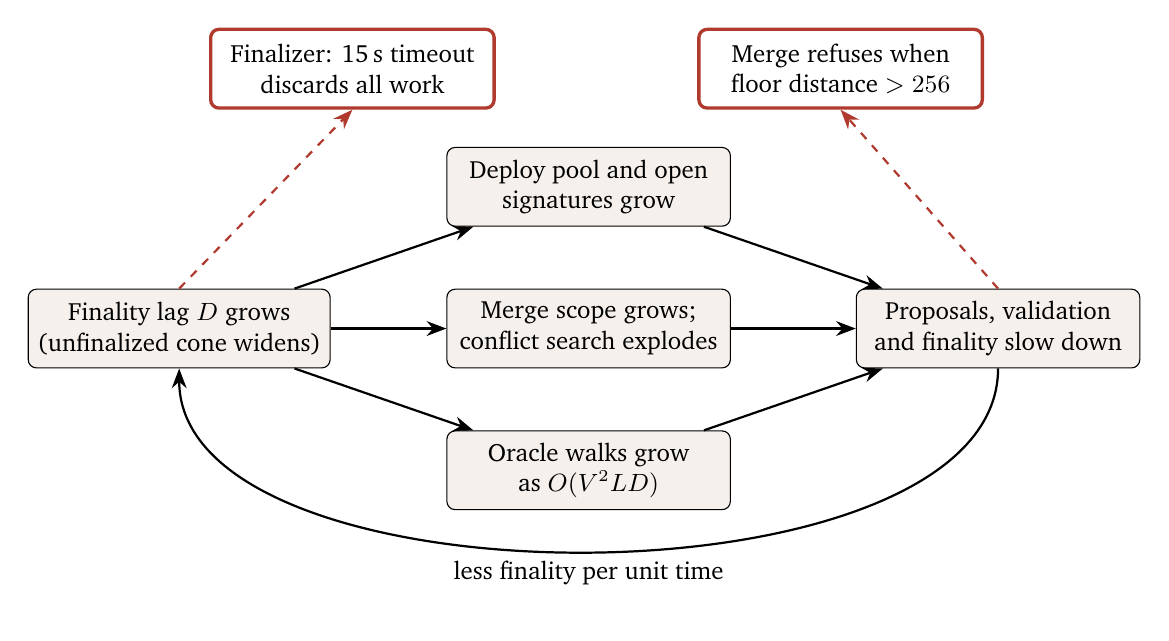
\begin{tikzpicture}[
  box/.style={draw,rounded corners=3pt,fill=soft,align=center,minimum width=3.6cm,minimum height=1.0cm,font=\small},
  trap/.style={draw=accent,very thick,rounded corners=3pt,fill=white,align=center,minimum width=3.6cm,minimum height=1.0cm,font=\small},
  arr/.style={-{Stealth[length=2.5mm]},thick}]
\node[box] (lag) at (0,0) {Finality lag $D$ grows\\(unfinalized cone widens)};
\node[box] (pool) at (5.2,1.8) {Deploy pool and open\\signatures grow};
\node[box] (merge) at (5.2,0) {Merge scope grows;\\conflict search explodes};
\node[box] (fin) at (5.2,-1.8) {Oracle walks grow\\as $O(V^2 L D)$};
\node[box] (slow) at (10.4,0) {Proposals, validation\\and finality slow down};
\draw[arr] (lag) -- (pool);
\draw[arr] (lag) -- (merge);
\draw[arr] (lag) -- (fin);
\draw[arr] (pool) -- (slow);
\draw[arr] (merge) -- (slow);
\draw[arr] (fin) -- (slow);
\draw[arr] (slow.south) .. controls (10.4,-3.6) and (0,-3.6) .. node[below,font=\small]{less finality per unit time} (lag.south);
\node[trap] (t1) at (2.2,3.3) {Finalizer: 15\,s timeout\\discards all work};
\node[trap] (t2) at (8.4,3.3) {Merge refuses when\\floor distance $>256$};
\draw[arr,accent,dashed] (lag.north) -- (t1.south);
\draw[arr,accent,dashed] (slow.north) -- (t2.south);
\end{tikzpicture}
\caption{The feedback loop. Every cost in the middle column grows with the finality lag. The two traps (outlined) turn the slowdown into a stop.}
\label{fig:loop}
\end{figure}

\subsection{Costs that grow with the lag, and the starvation paths}

\begin{itemize}
\item \textbf{Deploy pool.} About $8N$ signature checks per proposal for a pool of $N$, re-read under a lock.
\item \textbf{Lineage walks.} Quadratic in load: open signatures times segment length times deploys per block.
\item \textbf{Rejection-option search.} Exponential in conflicting pairs per group. Vault and PoS channels collapse groups into one, so the vault is a hot spot for the merge as well.
\item \textbf{Hot channels in RSpace.} $O(n)$ per touch and $O(n^2)$ over a run for a channel that accumulates $n$ datums. Replay scans its COMM list with a copy per step, $O(n^2)$ in COMMs (clone audit, finding~0.2).
\item \textbf{Finality walks.} $O(P \cdot V^2 L D)$ warm per block.
\item \textbf{Starvation.} A serial proposer queue, synchronous locks in async code, and CPU-bound consensus work on the async workers that also serve the network.
\end{itemize}

\subsection{Soak evidence}

The branch's proposal records two soaks. In August one merge call averaged 2.16\,s, 92\,\% of it settled-signature probes. In October no single stage separated failing sessions from passing ones, and the binding constraint had moved toward finality and Casper bookkeeping. The production high-phase replay targets recorded in \code{cost_accounting_perf_spec.rs} attribute about 229\,ms per deploy to precharge, 189\,ms to refund and 32\,ms to evaluation. That is, 93\,\% of replay time per deploy is spent moving money through the vault.

%======================================================================
\section{The blueprint: what the papers specify}\label{sec:blueprint}

This section reads the design from the papers. Each point ends with its consequence for the implementation.

\subsection{Signatures are names; token stacks are located terms}

The cost-accounted rho calculus extends names to $x, y ::= \lceil T \rceil \mid s$: signatures are channel names. Token stacks $S ::= () \mid s : S$ are first-class terms. Each layer is a balance cell of one signature. The companion paper refines the stack to a \emph{located} stack $S(I, s : S')$, a stack indexed by the surface $I$ that may draw on it. In rho this is a token stack sitting on a specific channel: only processes holding a matching channel name can consume from it. Unforgeable channels make that a genuine capability.

\emph{Consequence.} A signer's funds for computation are a stack on the signer's own channel in RSpace. They are not a balance in a shared contract.

\subsection{Payment is the communication}

The five rewrite rules are the COMM rule gated by token consumption. For a single signature,
\[
\{\, \mathtt{for}(y \leftarrow x)\,T \mid x!(U) \,\}_s \;\mid\; s : S \;\longrightarrow\; T\{\lceil U\rceil/y\} \;\mid\; S .
\]
The other four rules cover compound signatures and split or combined tokens. Joins follow one schema quantified over partitions, and conservation of authority holds across all of them: a join consumes exactly one receiver authority and one sender authority per channel.

\emph{Consequence.} The reducer charges by popping cells from located stacks. There is no separate settlement step that converts usage into money after the fact.

\subsection{Acceptance by linear proof is the concurrency control}

A deployment is accepted if and only if a linear proof of its resource use exists: for every signature $s$ it names, the supply $\Sigma_s$ meets the demand $\Delta_s$. The check runs before any step executes, and it is linear in the size of the AST. In the papers' words, two deployments competing for the same tokens are ``two proof obligations competing for the same linear hypotheses. At most one can succeed.'' Duplicate and simultaneous arrivals are resolved by the same rule, ``without locks, priority queues, or rollback mechanisms''.

\emph{Consequence.} Admission needs only the stacks of the envelope's own signers. Group decisions, later holds and shared cursors are unnecessary: committing tokens to an accepted deployment removes them from the supply that the next proof sees.

\subsection{Overcharge and refund}

Where control flow is data-dependent, the validator computes a conservative demand $\Delta^{\max}_c$, the maximum over reachable branches, and accepts if $\Sigma_c \ge \Delta^{\max}_c$. Execution consumes only the tokens it forces, and ``the residual $\Delta^{\max}_c - \kappa$ is returned to the client's token stack as part of the deployment's settlement''. The refund is safe because the number of tokens consumed equals the number of forced redexes, which the runtime counts exactly.

\emph{Consequence.} Settlement is a return of unused cells to the client's own stack. It is not a vault transaction.

\subsection{Located purses make the proof local}

Locating stacks decomposes the global resource obligation into one local linear proof per purse. The global proof is the separating conjunction of the local ones (companion paper, ``Local sufficiency composes''). Location also quarantines data-dependence to the surfaces that need a conservative bound.

\emph{Consequence.} The gate checks each signer's stack independently, and independent signers' checks can run concurrently.

\subsection{The cut is the one polymorphic constructor}\label{sec:polycut}

The companion paper presents a calculus's dynamics as an \emph{interaction cut}: an interaction constructor $K$ brings two introductions into contact, and a contraction computes the residual. In rho, $K$ is par. Every cost rule interposes a token between the operands of $K$ and drains it on contact. There is one $K$ per cut, so $K$ is the one constructor that must be made polymorphic: the outer $K$ combines a wrapped (signed) redex with a located purse, and the polymorphism of the introductions over their surface slots lets the whole-redex rule (R1) and the per-surface rules (R2, R3) coexist as one rule family. ``Meter the cut'' is the generic content of ``place valuable friction at every interaction''.

Two further properties follow from that construction. Wrapping is by construction, not by a dynamic operation: every continuation is a wrapped term, every redex lies inside a seal, and the cost steps only ever unwrap, so no redex can fire without consuming a token (the paper's no-leak corollary, a subject-reduction property). And iterated cost accounting flattens: nested seals multiply into a compound, so the cost construction is a monad, which is why nested signed terms flatten to $s_1 \otimes s_2$.

\emph{Consequence.} Cost accounting is one mechanism, parametric in what a stack holds. A located stack, its gating at the cut, the journal of its moves, its settlement and its conservation check are each written once, for every token kind. REV is one instance of that mechanism, distinguished only by policy: its kind name is held by genesis alone, so it is minted only at genesis (P2), it is the only staking token, and \code{phloPrice} is denominated in it. No part of the payment path may be written for REV in a way that a second kind must duplicate.

\subsection{Located stacks: authority named in the term}\label{sec:located}

A cost-accounted calculus makes the right to draw on a stack an authority, so the construction must not grant that authority silently: it must not introduce ambient authority. Whether proximity to a stack confers authority depends on the equational theory of $K$. When $K$ is free, position is unforgeable and the context next to a stack is itself the capability. As soon as $K$ carries any equation, an equation is a congruence step that changes adjacency without firing a cut or consuming a token, so a program can manoeuvre itself next to a stack it does not hold. Par is associative and commutative: the configuration is a freely mixed soup in which every process is adjacent to every stack. Taking proximity as authority in rho is exactly ambient authority, and it is the gap in the original cost-accounting paper that the companion paper closes.

The remedy is to carry the surface nominally. Interaction is gated on a nearness operator $\mathrm{near}(I,J)$ of the two surfaces, which in rho is name equality of subjects, and the stack is \emph{located} at the surface that may draw on it, $S(L, s : S')$ with $L = \mathrm{near}(I,J)$. Authority over a resource is then named in the term rather than conferred by the geometry of the bag: only a holder of a matching surface may compete for the stack. Nearness bounds competition without making it exclusive; exclusivity, where needed, is a matter for the type discipline and, here, for the gate.

\emph{Consequence.} Every authority to draw on, mint into or redirect a stack must be traceable to a surface named in the term: a signature that seals the redex, a channel name the term holds, an unforgeable name. It may never come from execution context (``whoever is running this deployment''), from adjacency, or from a privileged system name that any term can reach. Where the node checks the identity of the deployer or of a cosigner, that check is legitimate only as the verification of a seal that appears in the term, and must be written and tested as such (\S\ref{sec:authority}).

\subsection{Chains and antichains: where hot spots come from}

The spacetime paper maps a cost-accounted computation to a measured causal set. Events are COMM firings, the order is enabling, and concurrency is Bernstein independence of footprints: no write-write and no read-write overlap. Two of its results bear directly on throughput:
\begin{itemize}
\item \textbf{Time from the stack.} The firings that draw on a single located stack form a chain, ordered by stack depth. A shared stack, or any shared resource that every deploy writes, serializes every deploy that touches it.
\item \textbf{Space from the surfaces.} Firings that draw on distinct stacks at non-near surfaces are concurrent: they form an antichain.
\item \textbf{Number is volume.} The phlogiston spent equals the number of events, and discrete proper time is the longest chain.
\end{itemize}
With $W$ the total work and $L$ the longest chain, a scheduler on $P$ cores completes the work in at most $W/P + L$ (Brent's bound). Throughput therefore depends on keeping $L$ short: no state that every deploy writes.

\emph{Consequence.} A design meets the papers' throughput promise only if nothing on the payment path is shared across signers. A shared vault map, fee vault or cursor puts every settlement on one chain, and $L$ grows with $W$.

\subsection{Fees, minting, sponsors and multi-signature}

\begin{itemize}
\item \textbf{Fees.} In the worked example, the validator handler takes one token from the client's address $A_c$ and keeps it on its own fee channel $F_v$. The fee lands on a per-validator channel.
\item \textbf{Minting.} Minting is constructing a token stack and sending it on a signature channel. Epoch phlogiston for validators, slush funds and fee-to-stake conversion use the same primitive. Token creation is programmable: a contract may mint stacks of its own token kinds (Decision~28). The only restriction at this stage is that REV is the only staking token.
\item \textbf{Funding slots.} A contract creates an unforgeable channel and lets any funder deposit tokens on it. This decouples who authorizes, who pays and what runs. A sponsor funds a new user through a slot.
\item \textbf{Multi-signature.} A compound signature $s_1 \otimes s_2$ needs tokens from every component. Weakening is forbidden, so a compound token must be spent in full or explicitly split.
\end{itemize}

\emph{Consequence.} Sponsors, grants and owners are funding slots and located stacks, not post-run vault debits.

\subsection{Wallets disaggregated from the vault}

The located stack is how value is held, not only how fuel is held. A wallet is a stack of REV located on its owner's channel. The channel is a function of the owner's signature: a public key, an unforgeable name, or a compound signature for a multi-signature wallet. Finding a wallet is therefore a computation, not a lookup in a shared map. Only a term signed by the owner can draw on the stack. Anyone can deposit to it, as anyone can fund a funding slot.

Cells carry amounts. A balance is a count on a cell, not a list of unit cells, so spending splits a cell and receiving adds one. Deposits land as separate datums on the payee's channel and are combined only when the payee spends. Payments to one payee therefore commute: two deposits never conflict, and only spends from one wallet form a chain.

\emph{Consequence.} Moving REV is a COMM on the payer's and payee's channels. It needs no registry lookup, no map walk, no purse split through a shared mint and no settlement afterwards.

\subsection{Linearity: work happens because REV changes hands}\label{sec:linear}

In the calculus, linearity means that every token is consumed exactly once: forcing a signed redex pops one cell from a located stack, and the cell is gone. The monad paper reads that stack as the temporal monoid, a clock whose consumed prefix counts the steps run. Conservation of REV is an economic rule layered on top. The two fit together as two sorts:
\begin{itemize}
\item \textbf{Phlo is time.} It is ordered and consumed, and it is never commutative. It lives in the record, as the count $\kappa$ of work an envelope performed.
\item \textbf{REV is value.} It is spatial: deposits commute, nothing is lost, and the REV behind each consumed phlo moves to a counterparty. This is the paper's fee extraction, generalised so that all spending is payment for work.
\end{itemize}
Computation never creates or destroys REV, so the destination of consumed REV is not left open: the block or the genesis configuration names it.

Phlo is not a second currency. It is the rate at which REV in a wallet is spent: one phlo is \code{phloPrice} REV. Each COMM costs one phlo, and the schedule of Appendix~\ref{app:schedule} prices all other work in phlo. Nothing is minted per deployment and nothing is held in escrow. The REV stays in the wallet until work spends it.

A minimal example: client $c$ holds $r$ REV in its wallet $W_c$. Its deployment is one COMM, so $\Delta = 1$ phlo, at price $p$. Validator $v$ proposes the block that includes it.

\begin{Verbatim}[fontsize=\footnotesize,frame=single,framesep=6pt]
D  =  { x!(5) | for(y <- x) Nil }_c           -- one COMM, signed by c

block b, sender v, at D's canonical position:

  W_c!(r) | D                                -- c's wallet: r REV

gate:   r >= Delta * p = p                   -- accept; commit p against W_c
                                             -- (bookkeeping, nothing moves)

-> Rule 1, at price p (k = 1):
  { x!(5) | for(y <- x) Nil }_c | W_c!(r)
    ->  Nil | W_c!(r - p) | F_v!(p)          -- the COMM moves p REV from W_c to F_v

-> release the commitment (Delta - k = 0 unspent: nothing to return)

conservation:  (r - p) at W_c  +  p at F_v  =  r
\end{Verbatim}

The recipient is a name in the term, $F_v$, and $v$ is the block's sender. The term is fixed when $v$ proposes the block. Whoever reduces it, the runner or any replaying validator, reaches the same post-state, and appears nowhere in the term. Paying the runner would make executed state depend on who produced the record, not on the ordered blocks. So consumed REV moves to $F_{\mathrm{sender}(b)}$, and running and replaying are the work every validator does as a member of the shard.

Overcharge and refund keep their meaning without an escrow. The gate commits $\Delta^{\max} \times p$ against the wallet, and execution spends $\kappa \times p$. The residual $(\Delta^{\max} - \kappa) \times p$ never left the wallet, so the ``refund'' is the release of the commitment.

The second charge has the same shape. Work that is not a COMM (an addition, a method call, a substitution, the bytes of a send left in the tuplespace) is still work done under a signature, so it still moves REV. Its counterparty is not the proposer but the shard: a compute wallet named at genesis.

\emph{Consequence.} Conservation is an invariant of every block, and of the shard: the sum over wallets, validator channels and the compute wallet equals the genesis supply. There is no burn, no fixed fee and no mint of REV after genesis. Other token kinds, minted by contracts (Decision~28), are outside this sum and follow their issuers' rules.

\subsection{Internalisation}

The papers give a source-to-source translation of the cost-accounted calculus into pure Rholang~1.1, with splitter and joiner infrastructure. This gives cost-accounted semantics on today's runtime while the native implementation is built. The history-and-cost note adds that such an internalisation is lax: it carries an overhead grade. The native implementation is therefore the throughput path, and the translation is a bridge.

%======================================================================
\section{The gap, measured}\label{sec:measured}

\subsection{How the funding path works today}

The branch already has the papers' mechanism, but the v6 path does not use it:
\begin{itemize}
\item \textbf{Located stacks exist.} The reducer evaluates a token stack term by producing a \code{CostStack} datum on the signature channel of its head cell (\code{reduce.rs}, \code{eval_cost_stack}). The supply module models purse stacks and their inventory (\code{costacc/supply.rs}). Stack pops are accounted natively (\code{accounting/authority.rs}, \code{stack_pops}).
\item \textbf{v6 offers bypass them.} An owner-direct offer funds ``every class of the signer's own principal lane'' from the signer's vault (\code{owner_offer.rs}). The gate's supply ``counts SystemVault balances only'' (\code{gate.rs}). Fresh usage is bought from REV at the signed price on every deploy.
\end{itemize}

\begin{longtable}{@{}P{4.4cm}P{5.2cm}P{5.4cm}@{}}
\toprule
\textbf{Blueprint} & \textbf{Implementation (v6 path)} & \textbf{Measured effect} \\
\midrule
\endhead
Supply is the depth of the signer's located stack. & Supply is read from SystemVault balances through Rholang queries. & 44.5\,ms per balance query. The run phase spends 110--160\,ms beyond interpreting the term. \\
Payment is the COMM popping a cell. & The run is metered natively. The charge is then converted to REV and settled by \code{applyPhloCost}. & 560--600\,ms and about 1{,}000 events per envelope, under \code{Cost::unsafe_max()}. \\
Refund returns $\Delta^{\max} - \kappa$ to the client's stack. & \code{reserveAll}, \code{validateSettlement} and \code{settleReserved} run together after the run. & The reserve-and-refund happens, collapsed into one play after the run. \\
The linear proof is the concurrency control. & Holds that move no funds, plus \code{decide_groups}, \code{LaterHolds}, a held-capacity guard and the DR-28 cursors. & Settlement runs sequentially in block order. \\
Consumed REV moves to the counterparty; the system is linear. & \code{settleReserved} burns the resource charge, leaving it in a purse that nobody can reach. Only the fee moves. & REV is destroyed by computation, which breaks conservation. \\
A wallet is a located stack; moving REV is a COMM. & Wallets are purses in the vault's tree map, reached by registry lookup; a transfer runs the mint's split and deposit. & 81.6\,ms of contract code per user transfer. \\
The fee goes to the validator's own channel. & One fee vault, reached through \code{findOrCreate} by every settlement. & One write target shared by every envelope. \\
Distinct signers form an antichain. & Every settlement touches the vault map, the fee vault and the cursor map. & Settlement time per envelope grows with block size (Table~\ref{tab:blocks}). \\
The record carries the COMM log with charges. & The record also carries the wallet and receipt logs of the vault contracts. & About 92\,KB of a 100\,KB entry. \\
\bottomrule
\end{longtable}

\subsection{Measurements}

All figures come from release builds on the 2-vCPU host named on the first page, using tests in \code{casper/tests/v6_executor_spec.rs} and \code{casper/tests/util/rholang/cost_accounting_perf_spec.rs}.

\begin{table}[h]
\centering\small
\begin{tabular}{@{}rrrrrr@{}}
\toprule
\textbf{Envelopes} & \textbf{Runs} & \textbf{Settlement} & \textbf{Settlement share} & \textbf{Settlement per envelope} & \textbf{Envelopes/s} \\
\midrule
1 & 0.14\,s & 0.67\,s & 83\,\% & 0.67\,s & 1.24 \\
4 & 0.51\,s & 2.73\,s & 84\,\% & 0.68\,s & 1.24 \\
16 & 1.84\,s & 14.2\,s & 88\,\% & 0.89\,s & 1.00 \\
64 & 8.13\,s & 136.6\,s & 94\,\% & 2.14\,s & 0.44 \\
\bottomrule
\end{tabular}
\caption[Block execution by block size]{Block execution on the integration branch by block size (one-line sends from distinct payers; \code{phase_timings_by_block_size}). Settlement per envelope grows with block size, which is the mark of shared state.}
\label{tab:blocks}
\end{table}

\begin{table}[h]
\centering\small
\begin{tabular}{@{}lrrrr@{}}
\toprule
\textbf{Workload (one envelope)} & \textbf{Interpret term} & \textbf{v6 run phase} & \textbf{v6 settlement} & \textbf{Useful share} \\
\midrule
One send & 1.2\,ms & 112\,ms & 563\,ms & 0.17\,\% \\
256 sends & 29.7\,ms & 192\,ms & 605\,ms & 3.7\,\% \\
300 recursive COMMs & 32.5\,ms & 184\,ms & 572\,ms & 4.3\,\% \\
128 COMMs carrying 1\,KB each & 52.3\,ms & 211\,ms & 602\,ms & 6.4\,\% \\
REV transfer through the SystemVault & 81.6\,ms & --- & --- & --- \\
\bottomrule
\end{tabular}
\caption[Where the time of one envelope goes]{Where the time of one envelope goes (\code{cost_breakdown_of_one_envelope}, \code{a_user_vault_transfer_costs}). ``Interpret term'' is an unmetered exploratory run of the same term. Spawning a runtime costs 3.6\,ms and is subtracted.}
\label{tab:breakdown}
\end{table}

\textbf{Legacy \code{dev} pays the same cost.} The legacy precharge and refund system deploys, which also move REV through the vault, take 364\,ms and 291\,ms per deploy on the play path, against 0.3\,ms of evaluation. On replay, a block of seven deploys spends 106\,ms on precharge, 70\,ms on refund and 0.5\,ms on evaluation per deploy. The vault-centred payment path is the dominant per-deploy cost on both the legacy and the v6 path.

\textbf{System work is invisible to the meter.} The vault plays measured on October 28 report 0 phlo used under any budget. Work under the system signature is never drawn from a budget, so no allowance can bound it. Its event count is deterministic and linear in the number of sources: about 157 events (16\,KB) per source per play.

%======================================================================
\section{Design: cost-accounted order-then-execute on REV stacks}\label{sec:design}

\subsection{Principles}

\begin{enumerate}[label=P\arabic*.,leftmargin=2.2em]
\item \textbf{Wallets are located REV stacks.} REV lives on its owners' channels, disaggregated from the vault. A wallet's channel is computed from its owner's signature, so finding it needs no lookup. For a public key the channel is keyed by the key's REV address, which is what \code{wallets.txt} lists; an address cannot be inverted to a key, while a key always yields its address. Moving REV is a native operation on the payer's and payee's channels.
\item \textbf{REV is conserved.} REV is created once, at genesis, from the \code{wallets.txt} given to the shard. No later operation creates or destroys it.
\item \textbf{Phlo is a rate.} Work costs phlo, and a deployment's \code{phloPrice} says how much REV one phlo is. Phlo is never minted or held. Work moves REV from the paying wallet at that price.
\item \textbf{Two charges, two counterparties.} A COMM costs one phlo, which moves to the block's proposer. All other work under a signed term is priced by \code{dev}'s cost schedule, and moves to the shard's compute wallet.
\item \textbf{No shared state on a deploy's payment path.} Everything a deploy reads or writes to pay for itself is named by its own signatures: its wallets and its funding slots. The two exceptions are the proposer's channel and the compute wallet, where deposits commute and are combined once per block.
\item \textbf{Concurrency from independence.} Envelopes whose footprints are Bernstein-independent run concurrently. Conflicts are races on shared data channels, decided by the runner and recorded.
\item \textbf{Extension by hook, not by fork.} Behaviour beyond the core (rewards, staking shares, pricing policy) enters through hooks that default to no-ops and are replaced by contracts, under a multi-signature authority named at genesis.
\item \textbf{The consensus seam stays.} Order-then-execute, structural validity, the linearizer, records, attestation, inclusion checks, the finalizer design and backpressure are those of revision~2, as delivered in patches 0028--0035.
\item \textbf{One mechanism, parametric in the token.} Located stacks, gating at the cut, the journal of native moves, settlement and conservation are written once and parametrised by token kind (\S\ref{sec:polycut}). REV is the instance whose kind name genesis holds; it differs from other kinds by policy, never by code path.
\item \textbf{Authority is named in the term.} A stack may be drawn on, minted into or redirected only by a term holding a matching surface: a seal, a channel name or an unforgeable name (\S\ref{sec:located}). No authority comes from execution context, adjacency or a reachable system name; identity checks in the node exist only to verify seals that appear in the term.
\end{enumerate}

\subsection{Price and acceptance}

A deployment states \code{phloLimit}, the most phlo it may spend, and \code{phloPrice}, the REV it pays per phlo. These keep their meaning from \code{dev}, as D-12 requires.
\begin{itemize}
\item \textbf{The shard floor is a validity rule.} A block that includes a deployment priced below the shard's minimum price is invalid (block-validity step~8, preserved by D-12). The floor sits in the genesis policy.
\item \textbf{The validator's price is its own.} Above the floor, each validator decides the price at which it accepts deployments. A deployment below that price is simply not included by that validator. This is a market, not a consensus rule.
\item \textbf{The first version is a fixed price.} The node reads its acceptance price through a price hook. The first version of the hook returns a fixed price from the node's configuration. Making pricing programmable is a later change to the hook, with no change to consensus.
\item \textbf{One price for both charges.} The deployment's \code{phloPrice} prices COMMs and the rest of its work alike.
\end{itemize}

\subsection{The two charges}\label{sec:charges}

Work done under a signed term \signed{P}{s} is paid from the wallet at~$s$, at the deployment's \code{phloPrice}, in two ways.

\begin{center}
\small
\begin{tabular}{@{}P{3.2cm}P{5.3cm}P{3.0cm}P{3.6cm}@{}}
\toprule
\textbf{Charge} & \textbf{What it covers} & \textbf{Phlo} & \textbf{REV goes to} \\
\midrule
COMM & A redex that fires: a send meets a receive, or a join fires on all its channels & 1 per COMM & The block's proposer, $F_{\mathrm{sender}(b)}$ \\
Compute & Everything else $P$ does: evaluation of sends, receives, variables, \code{new}, \code{match} and \code{if}; arithmetic; method calls; substitution; and the storage of a send or receive left unmatched & \code{dev}'s cost schedule (Appendix~\ref{app:schedule}) & The shard's compute wallet, $W_{\mathrm{compute}}$ \\
\bottomrule
\end{tabular}
\end{center}

\textbf{Why two counterparties.} A COMM is the interaction that the block fixes, and its counterparty is the proposer that the block names (\S\ref{sec:linear}). Compute work has no such counterparty in the term: it is the cost to the shard of evaluating and storing what the term does. Its REV therefore goes to a wallet the shard holds. One compute wallet serves the whole shard; how its REV is later used (rewards, a share for stakers, a treasury) is a matter for the REV hook, which can move it but cannot create or destroy it.

\textbf{The compute wallet.} Genesis creates $W_{\mathrm{compute}}$ with a zero balance and places it under the hook authority: the same set of genesis addresses and the same threshold that replace hooks (\S\ref{sec:supply}). It is the one shared write target on the payment path. Deposits to it commute, and settlement combines each block's compute charges into one deposit, so it adds one datum per block, not one per envelope.

\textbf{Storage is charged once, when it is left.} \code{dev} charges a send or receive its storage size up front and refunds it when a COMM consumes it. The design keeps the sizes and nets the timing within the run:
\begin{itemize}
\item A send and a receive that meet within the envelope's run cost one phlo for the COMM and no storage.
\item A send or receive that the run leaves in the tuplespace, unmatched or persistent, pays its storage as compute: for a send, the bytes of its channel and data; for a receive, the bytes of its channels, patterns and continuation; and in both cases the event storage of $32 + 32k$ for $k$ channels. These are \code{dev}'s formulas (Appendix~\ref{app:schedule}).
\item When a later envelope consumes stored data, its COMM costs one phlo, and nothing is refunded. On \code{dev}, the consuming deploy is credited with the producer's storage refund. Here the producer's payment has already gone to the compute wallet, and a credit to another wallet would have to come from somewhere; so there is no cross-envelope refund.
\item \code{dev}'s COMM event-storage charge is replaced by the one phlo of the COMM.
\end{itemize}
This closes the payload-size gap: a send that carries a kilobyte and is left in the tuplespace pays for the kilobyte. Charging stored data again over time, in units of block time, is rent; it is left to a later revision.

\textbf{What stays uncharged.} File I/O (\code{rho:io:fs:native:*}), whose weights \code{dev} defines but discards, and the spatial matcher, which \code{dev} never charged, stay uncharged in this revision. Appendix~\ref{app:schedule} lists them with the other flat-priced operations as known gaps.

\textbf{Who pays.} The wallet at the signature of the signed term whose work it is:
\begin{itemize}
\item A deployment with no explicit wrapper is \signed{D}{deployer}. Parsing the deployment's source happens outside any wrapper and is charged to the deployer.
\item Uniform signing, \signed{for(y <- x) P}{s}, charges both the COMM and the continuation's compute to~$s$.
\item The linear transfer \signed{for(y <- x) P}{s1 -o s2} charges the COMM to $s_1$ and the continuation's compute to $s_2$.
\item Nested wrappers flatten to the compound $s_1$~\texttt{(*)}~$s_2$, as the cost monad's multiplication requires.
\item A compound signature does not split the charge. Under \signed{P}{s1 (*) s2} the wallets at $s_1$ and at $s_2$ each pay the full charge for $P$'s work: each COMM costs each of them one phlo, and each compute charge falls on each of them in full, at the deployment's \code{phloPrice}. With $n$ components the work is paid $n$ times. The excess is the cost of coordination: joint authority is something every party buys. It matches the paper's Rule~2, in which every component supplies its own token to each COMM, and weakening stays forbidden, since no component can be left out.
\item A joint wallet, located at the compound signature $s_1$~\texttt{(*)}~$s_2$ itself (a multi-signature wallet), pays once, as the single combined token does in the paper's Rule~3.
\end{itemize}
For a compound signature, the gate checks each component's wallet separately: each must cover the full commitment, $\Delta \times {}$\code{phloPrice}, and each gets its own entry in the commitment table. Settlement credits the proposer once per component for COMMs, and the compute wallet once per component for compute. More REV moves, but none is created or destroyed, so conservation holds.

\textbf{Sharing the cost of coordination.} Since \code{phloPrice} is set by the deployment, coordinating parties can lower what they pay: two parties deploying at half the usual price together pay what one would pay at the full price. The shard's price floor (\S\ref{sec:supply}) is not scaled by the number of components. This is by design: it sets a minimum coordination cost, so $n$ parties together never pay less than $n$ times the floor price. The lower price applies to the whole deployment, and a validator may include lower-priced deployments later.

\textbf{Contracts that pay for themselves.} A signed term may name the hash of a process, \signed{P}{\# P}, so that a contract pays for its own work from the wallet at its hash. That wallet is debited only by the work of $P$ itself. Anyone may deposit to it, as anyone may fund a funding slot, and each deposit is recorded against the funder's address. Sending REV is less dangerous than drawing it, but it raises one problem: a contract doing harm can be kept running by whoever keeps funding it. Defences that name the bad party do not hold, because names are cheap: a trivially changed $P$ has a new hash and a new wallet, and a new address is one key pair away. What is not cheap is REV, which is conserved, and capabilities, which are unforgeable names. The defences are aimed at those, in order:
\begin{enumerate}
\item \textbf{Revoke the interaction, not the funding.} $P$ causes harm only through COMMs, which need counterparties on channels $P$ can reach. The parties that granted those unforgeable channels revoke them with the usual object-capability patterns, a caretaker or a membrane they can cut. Money cannot buy a capability back, and a rehashed $P$ holds none of the old one's names. A contract that no one will talk to only turns its funders' REV into payments to proposers and the compute wallet.
\item \textbf{Refuse a funder's share.} Since deposits are recorded per funder, a funder's unspent contribution to \texttt{\# P} can be refused without touching anyone else's. New identities still get through, but each attempt costs real REV and leaves a record for remedies off the chain.
\item \textbf{Refuse by behaviour, as a last resort.} The hook authority may register a spatial-behavioural formula. The gate refuses commitments against any \texttt{\# P} whose $P$ satisfies it; the check runs once per hash and is cached, off the hot path. A new hash does not evade a formula about behaviour; evasion means disguising the behaviour itself. A list of banned behaviours can be dodged, while admitting only behaviours proven safe cannot be, at the price of refusing some honest contracts; the choice is the authority's. Refusal never moves REV, deposits are still accepted, and every formula is published on the chain, so the policy is visible and open to dispute.
\end{enumerate}
The behavioural refusal sits behind the REV hook and, like every hook, is a no-op by default.

Phase~2 admits only the deployer's own signature in the signed terms of a deployment (\S\ref{sec:plan}); funding slots, owners and compound signatures follow in phase~3.

\subsection{The annotation syntax}\label{sec:syntax}

The surface syntax is the paper's concrete syntax (Appendix~C of the cost-accounted rho paper), already implemented in two places:
\begin{itemize}
\item \textbf{Parser.} \code{F1R3FLY-io/rholang-rs}, branch \code{feature/cost-accounting-transpiler} at \code{02cef80}: the forms \signed{P}{s}, \texttt{s :: S}, \texttt{\# P}, \texttt{s1 (*) s2}, \texttt{s1 -o s2} and the per-clause signed bind, with an AST, a corpus and golden tests. It is not on \code{rholang-rs} master; \code{dev} pins \code{527af8a}, which has none of it.
\item \textbf{Normalizer.} \code{feature/cost-accounted-rho}, \code{compiler/normalizer/cost_accounting/} (about 450 lines): recognition of signed terms and stacks, the uniform-signing and lollipop desugarings, flattening of nested signatures to a compound, and the guard against cost syntax in patterns. It lowers signed terms to \code{CostSignedTerm} and stacks to \code{CostStack} in the protobuf model.
\end{itemize}
The design ports the parser and the normalizer as they are, and re-implements the reducer's part on the native REV layer rather than porting the branch's 4{,}952-line \code{authority.rs}:
\begin{itemize}
\item A signed term opens a funding region for its signature; COMMs and compute inside it are charged to that region's wallet.
\item A stack literal \texttt{s :: S} of REV is a native transfer from the writer's wallet onto the signature channel, never a mint. This is what the branch's \code{eval_cost_stack} does, and conservation requires it.
\item Token creation is otherwise programmable (Decision~28), and token kinds are instances of the same mechanism, not a second one (P9). A token kind is named by an unforgeable name held by its issuing contract. A stack of a kind is written as a stack signed for that kind: signed with the kind's name it is a mint, which only the holder of the name can write; signed with a read-only bundle of the name it is a transfer from the writer's stack of that kind (Decision~42). REV is the kind whose name genesis holds, so no contract can mint REV. Only REV is a staking token, and charges stay in REV, since \code{phloPrice} is REV per phlo. Wallets of every kind are located stacks keyed by owner and kind; the journal records moves and mints as one entry type parametric in kind; conservation is checked per kind, and for REV against the genesis supply (Decision~46).
\end{itemize}

\subsection{The life of an envelope}

\begin{Verbatim}[fontsize=\footnotesize,frame=single,framesep=6pt]
gate(e, R, C):                    -- in block order, at the block pre-state R
  Delta = demand of e in phlo: COMMs + compute (Delta_max where data-dependent),
          <= phloLimit
  for each wallet w that e's signers fund it from:
    need_w = w's share of Delta * phloPrice
    have_w = REV on w's located stack at R  -  C[w]     (native read)
  accept iff have_w >= need_w for every w               (one local proof per purse)
  on accept: C[w] += need_w                             (commitment: bookkeeping)
run(e):                           -- concurrent with the other envelopes
  per wallet w, count k_comm[w]: one phlo per COMM, under rules 1-5 and joins
  per wallet w, count k_compute[w]: phlo of the cost schedule, including the
                storage of what the run leaves in the tuplespace
settle(e):                        -- in block order, after the merge
  debit each w by (k_comm[w] + k_compute[w]) * phloPrice, in canonical form
  credit F_sender(block) with sum k_comm * phloPrice
  credit W_compute       with sum k_compute * phloPrice
  release C[w] for e's wallets    (the unspent (Delta - k) * phloPrice never left)
  exhausted (signed limit reached): k = phloLimit, so the whole commitment
                is spent, each phlo to the counterparty of its work
end of block:  combine the block's credits into one deposit on F_sender(block)
               and one on W_compute; run the REV hook; check conservation
\end{Verbatim}

\begin{itemize}
\item \textbf{Native, not Rholang.} The wallet read, the commitment, the debits and the deposit are runtime operations on signature channels. They run no contract code and leave no Rholang event log.
\item \textbf{The commitment is the reservation.} The commitment table $C$ belongs to the block's execution, not to RSpace. Gating runs in block order, so a later envelope that draws on the same wallet sees the earlier commitments, and the sum of commitments on a wallet never exceeds its balance. Every block settles all of its envelopes, so no commitment outlives its block. Replay reproduces $C$ from the gate verdicts in the record.
\item \textbf{The overestimate bounds the commitment.} With a complete proof the commitment is $\Delta \times$ \code{phloPrice}, often far below \code{phloLimit} $\times$ \code{phloPrice}. With an incomplete proof it is the signed limit, exactly as in \code{dev}. The linear proof bounds the COMM part of $\Delta$; until a static estimate of the compute part exists, the compute part is bounded only by \code{phloLimit}, so $\Delta = $ \code{phloLimit} in practice.
\item \textbf{Exhaustion.} An envelope that reaches its signed limit stops. It has then spent its whole commitment, and each phlo has already gone to the counterparty of the work it paid for. Revision~5's rule that an exhausted envelope's full commitment goes to the proposer is no longer needed.
\end{itemize}

\subsection{Box-car batching and the canonical form}\label{sec:boxcar}

Writing a wallet debit for every COMM is wasteful when an envelope makes thousands of them. Each node may therefore batch its debits, with a box-car size set in the node's configuration. Batching is a matter of how one node schedules its writes, so it must not change the state that consensus sees. Two nodes with different box-car sizes must reach the same state root. The design guarantees that with one rule:

\begin{keypoint}
\textbf{Canonical settled form.} After a block settles, each wallet that paid holds one combined datum, its balance less $(\kappa^{\mathrm{comm}}_w + \kappa^{\mathrm{compute}}_w) \times$ \code{phloPrice} summed over the block's envelopes; the proposer's channel holds one new deposit datum for the block's COMM charges; and the compute wallet holds one new deposit datum for the block's compute charges. Intermediate debits are not part of the state. A term that reads its own wallet during its run sees the pre-state balance less the commitments recorded against that wallet up to and including its own gate position, which is also independent of the box-car size.
\end{keypoint}

The record carries $\kappa^{\mathrm{comm}}_w$ and $\kappa^{\mathrm{compute}}_w$ per wallet, so replay checks the settled form, not the write schedule. The box-car size is a per-node parameter, as decided. It affects how fast a node runs, and it never affects the state.

\subsection{REV transfers}

A transfer from wallet $A$ to wallet $B$ is a deployment signed by $A$. Its few COMMs cost phlo like any other deployment's. The movement of REV is one native debit of $A$'s stack and one native deposit on $B$'s channel. Deposits land as separate datums, so transfers to one payee never conflict, and transfers between disjoint pairs run concurrently. Only spends from one wallet form a chain, and the linear proof already orders those.

The SystemVault stops being the custodian of REV. At most it remains as a compatibility facade: \code{find} returns the wallet channel, and \code{transfer} is the native transfer.

\subsection{Supply and hooks}\label{sec:supply}

\begin{itemize}
\item \textbf{Genesis.} Genesis creates one located stack per line of \code{wallets.txt}, keyed by that line's REV address, with that balance, and an empty compute wallet. This is the only creation of REV. Every block's executor checks that the sum over wallets, validator channels and the compute wallet equals the genesis supply. The check is incremental: each block's debits and credits sum to zero, with an occasional full audit.
\item \textbf{The REV hook.} Genesis installs a hook that is called at fixed points (after each block's settlement, and at epoch boundaries) and does nothing. Rewards, sharing a proposer's receipts with its stakers or delegators, or any other policy are contracts that replace the no-op. A hook can move REV but cannot create it, because conservation is checked after it runs.
\item \textbf{The price hook.} As above: the first version returns the node's fixed price.
\item \textbf{Hook authority.} Genesis names a set of addresses and a threshold. Replacing a hook is a deployment signed by at least the threshold of those addresses (a compound signature over them). No other signer can change a hook.
\item \textbf{The compute wallet's authority.} The same addresses and threshold hold the compute wallet. Spending from it is a deployment with that compound signature, or the work of a hook they installed. A single compute wallet per shard is the default; splitting it (per epoch, or per proposer) is a change to the REV hook, not to consensus.
\end{itemize}

\subsection{Mechanisms that must justify their authority}\label{sec:authority}

P10 is checked mechanism by mechanism. Each item below moves, mints or redirects value, and each must show the surface in the term from which its authority comes. Until an audit has done so, each is a risk (\S\ref{sec:risks}).
\begin{itemize}
\item \textbf{The native wallet process} (\code{rho:rev:wallet}). A transfer draws on the wallet located at the payer's signature. Its authority is the payer's seal on the deployment (or, for a compound payer, every component's seal). A version that accepted any deployer id as payer was an ambient-authority leak and has been closed (P3-02).
\item \textbf{The bond process} (\code{rho:rev:bond}). Bonding draws on the validator's own wallet under its seal; release and slashing redirect bond REV and must be reachable only through the PoS contract's own unforgeable names, not by any term that can name the process.
\item \textbf{The genesis mint} (\code{rho:rev:genesis}) and the reducer's genesis-only URN filter. The only creation of REV; its authority is genesis itself, and the filter must make the process unreachable from any later term.
\item \textbf{Cosigner names} (\code{rho:system:cosignerId:<i>}). A name for a seal carried by the envelope; it confers authority only because the cosignature over the envelope's bytes is verified.
\item \textbf{The system authorization token}. Held only by system deploys; it must remain an unforgeable name that no user term can obtain.
\item \textbf{Signatures named in signed terms} (\code{GateInput.named}) and the reducer's runtime check. These verify that every seal in the term is held by a signer of the envelope; they are the node's side of the nominal surface, not a source of authority in themselves.
\item \textbf{The native journal}. Moves recorded during a run are applied at settlement; an entry may name only stacks the run had authority over when it recorded the entry, and the entry type is parametric in kind.
\end{itemize}

\subsection{Owners, sponsors and grants}

\begin{itemize}
\item \textbf{Owners} (DR-135) pay for the regions of their stored processes at their own price, from their own REV wallets. An owner without the REV refuses the introduction, as the branch's region refusal already does.
\item \textbf{Sponsors} use funding slots: an unforgeable channel holding deposited REV, named by the deploy that it funds.
\item \textbf{Grants} are funding slots with a validity window that the gate checks at block time.
\end{itemize}

\subsection{Block execution}

\begin{enumerate}
\item \textbf{Gate} every envelope at $R_0$, in block order, accumulating commitments. The wallet reads are independent per wallet and run concurrently. The commitment accumulation is a pass over a table in memory.
\item \textbf{Run} every admitted envelope concurrently from $R_0$.
\item \textbf{Merge} in block order. A conflicting envelope is rolled back and keeps its charge for the run, as decided on October 25.
\item \textbf{Settle} in block order, natively, in the canonical form of \S\ref{sec:boxcar}: debit the wallets, then make one deposit to the proposer and one to the compute wallet. Run the REV hook. Check conservation.
\end{enumerate}
The ordered steps (1 and 4) are cheap. The expensive step, the run, is the concurrent one.

\subsection{Records}

A record entry carries the gate verdict and commitment, the outcome, the COMM phlo and the compute phlo spent per wallet, the REV moved to the proposer and to the compute wallet, the budget recording and operation journal needed for replay, and the user COMM log. It carries no system log. With the 0035a analysis of 1.25 bytes of user log per phlo (0.1 measured), an entry is at most $1.25\,\Delta + r_0$ bytes, with $r_0$ under 4\,KB measured. A per-block demand cap $D$ with $1.25\,D + E\,r_0 \le$ \code{block-record-bytes} then guarantees that every record can be cited. That closes the liveness hole of 0035 by arithmetic alone, and citing records in pieces (0035b) is no longer needed. The 1.25 bytes per phlo was measured under the old units; with storage now priced by the byte, a large payload costs phlo in proportion to its size, which can only lower the bytes of log per phlo, but the ratio is re-measured in phase~2 before the cap is fixed.

\subsection{What leaves the execution path}

\begin{itemize}
\item The SystemVault as custodian of REV, its tree map of purses, its registry lookup and its mint-based purse split.
\item The precharge and refund system deploys, the settlement call \code{applyPhloCost}, its unlimited budget, its burn of the charge, and its logs in the record.
\item Vault reads in the gate. Supply becomes a wallet balance read natively.
\item Holds as fit checks, \code{decide_groups}, \code{LaterHolds} and the held-capacity guard.
\item The DR-28 monetary cursors and their vault validation, and with them the reason for the DR-119 bucket locks.
\item The shared fee vault and the fixed fee. The compute wallet is not a fee vault: it receives one deposit per block, at settlement, and no envelope reads it.
\item \code{dev}'s cross-deploy storage refunds and its COMM event-storage charge (\S\ref{sec:charges}).
\item The vault-based precharge and refund of October 28 (withdrawn before merge).
\end{itemize}

There is no legacy chain to preserve. This is software from which others build blockchains, and no deployed shard depends on the vault-based path. The rule of revisions 2 to 4, that legacy paths stay byte-identical to \code{dev}, is relaxed. Code on the old path is removed where removing it is simpler than keeping it. There is no migration of balances.

%======================================================================

\section{Throughput analysis}\label{sec:throughput}

\subsection{Model}

Let an envelope's core time be the sum of four parts: its interpretation $u$, the metering overhead factor $m$ on that interpretation, its funding work $f$ (wallet read, commitment, debits and the proposer deposit), and its share $c$ of the block's checkpoint and merge. On $P$ cores with parallel efficiency $\eta$, and with the longest chain $L$ short relative to the work, node throughput is
\[
X \;\approx\; \frac{\eta\,P}{m\,u + f + c}.
\]
Every validator executes or replays every block, so shard throughput equals the throughput of one node. Adding validators adds safety, not throughput.

\textbf{Today.} $f$ is the run-phase funding overhead (110--160\,ms) plus settlement (560--600\,ms), and settlement is one chain. The parallel term does not apply to it, and its per-envelope cost grows with block size. A REV transfer adds 81.6\,ms of vault contract code on top.

\textbf{Design.} $m = 1.2$, from the branch's own profiles (15--23\,\% more CPU in the reducer). The funding work $f$ covers a native wallet read, the commitment, the debits in canonical form, the proposer deposit and the gate's linear estimate. The checkpoint share is $c \approx 0.5$\,ms (31\,ms per 64-envelope block measured). Together $f + c$ is taken as 2 to 8\,ms, with 5\,ms as the middle value. A REV transfer adds one native debit and one native deposit, taken as 0.5 to 2\,ms. These ranges are estimates until phase~2 measures them. Without the escrow moves and the mint of revision~4, $f$ should sit in the lower half of its range.

\textbf{The second charge.} Pricing compute adds no interpreter work: \code{dev}'s meter already evaluates the schedule on every operation, and $m$ includes it. It adds two counters per paying wallet, and one deposit to the compute wallet per block rather than per envelope, so its share of $f$ is negligible. The figures below are unchanged from revision~5.

\subsection{Per-envelope work}

\begin{table}[h]
\centering\small
\begin{tabular}{@{}lrrrr@{}}
\toprule
\textbf{Workload} & \textbf{Today} & \textbf{Design (range)} & \textbf{Gain, middle} & \textbf{Gain, range} \\
\midrule
One send & 675\,ms & 6.4\,ms (3.4--9.4) & 105$\times$ & 72--198$\times$ \\
REV transfer & 756\,ms & 7.4\,ms (3.9--11.4) & 102$\times$ & 66--194$\times$ \\
256 sends & 796\,ms & 40.6\,ms (37.6--43.6) & 20$\times$ & 18--21$\times$ \\
300 recursive COMMs & 756\,ms & 44.0\,ms (41.0--47.0) & 17$\times$ & 16--18$\times$ \\
128 COMMs carrying 1\,KB & 813\,ms & 67.8\,ms (64.8--70.8) & 12$\times$ & 11--13$\times$ \\
\bottomrule
\end{tabular}
\caption{Core time per envelope, today (run phase plus settlement, single-envelope block; for the transfer, plus the measured 81.6\,ms of vault code) and projected. A transfer's own COMMs are taken as a one-send deployment. The gain is largest where the deploy does least, because today's cost is almost all funding overhead.}
\label{tab:gain}
\end{table}

\subsection{Node throughput}

\begin{table}[h]
\centering\small
\begin{tabular}{@{}lrrrr@{}}
\toprule
\textbf{Workload} & \textbf{2 cores} & \textbf{8 cores} & \textbf{16 cores} & \textbf{32 cores} \\
\midrule
One send & 187--281 & 750--1{,}124 & 1{,}499--2{,}249 & 2{,}998--4{,}497 \\
REV transfer & 162--243 & 648--972 & 1{,}297--1{,}945 & 2{,}593--3{,}890 \\
256 sends & 30--44 & 118--177 & 236--354 & 472--709 \\
300 recursive COMMs & 27--41 & 109--164 & 218--327 & 436--655 \\
128 COMMs carrying 1\,KB & 18--27 & 71--106 & 142--213 & 283--425 \\
\bottomrule
\end{tabular}
\caption{Projected envelopes per second for one node, with parallel efficiency $\eta$ from 0.6 to 0.9, for envelopes with independent signers and no shared data channel. Today's measured rate on the same 2-core host is 0.44 (64-envelope blocks) to 1.24 (single-envelope blocks). Absolute values are for the measurement host. Faster hosts scale all figures alike, today's included.}
\label{tab:throughput}
\end{table}

\textbf{Reading the tables.} On 2 cores, the design projects 150--640 times today's measured rate for one-line deploys, and 130--550 times for REV transfers, against 1.24 envelopes per second for single-envelope blocks and 0.44 for 64-envelope blocks. For the heavier workloads it projects 14--36 times their single-envelope rate of 1.2--1.3 per second. On 16 cores, with independent signers, the factors become about 1{,}050--5{,}100 for small deploys and transfers, and 110--290 for the heavier ones. The gain has two sources that multiply: removing fixed funding overhead and the vault (Table~\ref{tab:gain}), and replacing one causal chain with an antichain, so that cores apply (Table~\ref{tab:throughput}).

\subsection{Where the anticipated gains do not appear}\label{sec:limits}

The model supports large gains for overhead, payments and concurrency. It does not support them unconditionally. These are the cases where it projects less, and why.

\begin{enumerate}
\item \textbf{Deploys dominated by their own computation.} The gain is $(m\,u + f_{\mathrm{today}})/(m\,u + f)$. For a deploy that interprets for 50\,ms it is about 12, and it falls toward 1 for very heavy deploys. Against the unmetered legacy path it falls toward $1/m$, below 1. The design removes overhead. It does not make Rholang faster, and the metering factor $m = 1.2$ is a real cost. The interpreter's own defects (clone audit, Tier~0: quadratic \code{Env::put}, quadratic replay scan, quadratic \code{eval_match}) are separate wins of 2.7--273 times on the patterns they affect.
\item \textbf{Application hot channels.} Two deploys that write the same data channel, such as a popular contract's state or a liquidity pool kept in one contract, form a chain. If a fraction $h$ of the work lies on one chain, Amdahl's law limits the speedup on $P$ cores to $1/(h + (1-h)/P)$. On 16 cores, $h$ of 1, 5, 10 and 25\,\% gives 13.9, 9.1, 6.4 and 3.4. The design removes the system's hot spots, including the vault. Applications can still create their own.
\item \textbf{One busy wallet.} All spends from one wallet form a chain, by the papers' own result. A single account that submits most of the load is serialized at its precharge. The precharge is cheap, but the order is fixed. Deposits to one wallet do not have this limit, because they commute.
\item \textbf{The consensus cap.} A block carries at most $E = 256$ envelopes, and blocks execute in canonical order. Shard throughput is at most $E \cdot V \cdot r$ for $V$ validators proposing $r$ blocks per second: 768 per second for three validators at one block per second, 1{,}536 for six. For small deploys and transfers this cap binds before 16 cores do. Raising it means a larger $E$ (bounded by the record arithmetic above), faster proposals, or executing blocks with disjoint footprints concurrently (refinement R1).
\item \textbf{Replication.} Every node executes or replays every block, so validators add no throughput. Replay is cheaper than execution, with no matching search, but still proportional to the work.
\item \textbf{Multi-core efficiency is not measured.} The range $\eta = 0.6$--$0.9$ is an assumption. On today's code, the run phase's core time per envelope grows from 140\,ms alone to 254\,ms in a 64-envelope block on 2 cores. Part of that is vault reads in the gate, which the design removes, and part may be contention in RSpace's hot store. Until the phase~2 scaling run measures it, the 8- to 32-core columns are projections, not results.
\item \textbf{The funding work estimate.} The 2--8\,ms for native funding work and the checkpoint share is an estimate from RSpace operation costs. If native stack operations cost as much as Rholang COMMs (about 1\,ms each, measured in the legacy reducer breakdown), $f$ approaches the top of its range and the one-send gain falls toward 72 times.
\end{enumerate}

\subsection{Validation}\label{sec:validation}

These measurements turn the projections into exit criteria:
\begin{itemize}
\item \textbf{Funding microbenchmark (phase~2).} The gate, commitment, debits and settlement for one envelope funded from one to four wallets. Target: under 8\,ms on the measurement host.
\item \textbf{Transfer benchmark (phase~2).} A REV transfer between two wallets as a deployment, end to end. Target: under 12\,ms per transfer on the measurement host, and at least 150 transfers per second on 2 cores with independent payers.
\item \textbf{Block benchmark (phase~2).} \code{phase_timings_by_block_size} and \code{cost_breakdown_of_one_envelope} rerun on the new path. Targets: settlement under 5\,\% of block time, settlement per envelope flat in block size (within 20\,\% from 1 to 64 envelopes), and one-send throughput of at least 150 per second on 2 cores.
\item \textbf{Scaling run (phase~2).} The same block benchmark on 8 and 16 cores. Target: $\eta \ge 0.6$. A lower result points to RSpace contention and opens a work item.
\item \textbf{Conservation.} Every executor and benchmark run checks that the sum over wallets, validator channels and the compute wallet equals the genesis supply after each block, and that replay reaches the same root for different box-car sizes.
\item \textbf{The compute charge (phase~2).} On a corpus that exercises every row of Appendix~\ref{app:schedule}, the compute phlo recorded per wallet equals the schedule's figure, in play and in replay; matched sends pay no storage, unmatched and persistent ones pay theirs once.
\item \textbf{B7 soak.} Sustained throughput against a legacy soak on the same hardware, with the hot-channel workloads of item~2 above as a separate profile.
\end{itemize}
\section{The path to a working branch}\label{sec:plan}

This section answers one question: what is the quickest path to a working branch that carries the full implementation and can be merged back to \code{dev}? It reviews current \code{dev}, the Track~A changes and the integration branch against the design of \S\ref{sec:design}, and proposes a base and a sequence of phases.

\subsection{Where the code stands (October 29, 2026)}

\begin{longtable}{@{}P{3.4cm}P{11.6cm}@{}}
\toprule
\textbf{Line of work} & \textbf{State} \\
\midrule
\endhead
\code{dev} & At \code{252a86d1d} (October 28), 583 commits past the point where Track~A forked on October 16. It has landed its own versions of several Track~A fixes: oracle verdicts shared within a floor derivation with the validated floor kept (near A1a), a reused pool snapshot during block creation and mutex-free pool storage (near A4), the unfinalized cone walked over cached block facts (near A5), the finalizer as the single writer of the LFB with one finalizer task per Casper instance, and the re-fetch rate limit (equivalent to A7). \\
Track~A (A1a--A9) & Not on \code{dev}. Three branches in series: \code{fix/finality-stall-track-a} (A1a, A2, A3), \code{fix/finalizer-forward-progress} (A1b, A1c) and \code{fix/stall-track-a-rest} (A4--A9), 67 files, about 4{,}100 lines added. \\
Integration branch & \code{integration/cost-accounted-ote-b1d866e45} at \code{d1f3ab5e1}: Track~A, the cost-accounting work of \code{feature/cost-accounted-rho}, and the v6 seam through patch 0035. About 230{,}000 lines added, 534 commits behind \code{dev}, with 105 files that \code{dev} has also changed. \\
v6 seam & Canonical order, structural validity, the linearizer, records, attestation, the executor, pruning, the lag gate, inclusion checks and A-LIN: about 6{,}400 lines on the integration branch, mostly self-contained. Eight of its 21 files import from \code{costacc}, one or two lines each: the genesis resource policy (five uses), the executor's run types from \code{direct_wallet_funding}, the owner offer in proposal, and the close-block deploy. Only \code{rho_settlement.rs} is wholly tied to the old funding path. Its original form, \code{feature/cost-accounted-ote}, is 2{,}600 lines on an older \code{dev}. \\
P1 (vault precharge and refund) & Withdrawn, uncommitted, not to ship. \\
Annotation syntax & Parser on \code{rholang-rs} \code{feature/cost-accounting-transpiler} at \code{02cef80}, not on its master; \code{dev} pins \code{527af8a}, without it. Normalizer, protobuf messages and reducer support on \code{feature/cost-accounted-rho} only. Not on \code{dev}, \code{feature/cost-accounted-ote} or the v6 seam. \\
Cost schedule & On \code{dev}, in \code{accounting/costs.rs} and the reducer (Appendix~\ref{app:schedule}). File-I/O weights defined but discarded by \code{NoopMetering}. \\
\bottomrule
\end{longtable}

\subsection{Trial merges}

\begin{longtable}{@{}P{5.2cm}P{9.8cm}@{}}
\toprule
\textbf{Trial} & \textbf{Result} \\
\midrule
\endhead
All of Track~A into current \code{dev} & Conflicts in 15 files. The heaviest are \code{block_creator.rs} (9 hunks) and \code{finalization_runner.rs} (7). The rest are \code{casper.rs}, \code{block_admission.rs}, \code{types.rs}, \code{deploy_lifecycle.rs}, the Casper buffer store, metrics constants, five API and bonding tests, \code{test_node.rs} and \code{supply-chain/policy.toml}. \\
Track~A one commit at a time & A2, the \code{commit_lfb} part of A1c, A6 and A8 apply cleanly, in that order: A8's tests use \code{commit_lfb}, so A8 conflicts if applied before A1c. A1a, A1b, the floor cursor, A3, A4, A5, A7 and A9 conflict. Most of those conflicts come from \code{dev}'s overlapping fixes, not from logic that disagrees. \\
\code{feature/cost-accounted-ote} into current \code{dev} & Conflicts in 9 files: \code{casper.rs}, \code{finalization_runner.rs}, four API tests, the bonding spec, \code{test_node.rs} and \code{supply-chain/policy.toml}. These are mostly constructor and test-harness signatures. \\
Integration branch into current \code{dev} & Not attempted in full. With 105 files changed on both sides and 534 commits of drift, the conflicts would fall largely in code that this design deletes. \\
\bottomrule
\end{longtable}

\subsection{The choice of base}

\begin{longtable}{@{}P{3.0cm}P{6.0cm}P{6.0cm}@{}}
\toprule
& \textbf{Current \code{dev} + reduced Track~A} & \textbf{Continue the integration branch} \\
\midrule
\endhead
Drift from \code{dev} & None at the start; each phase rebases cheaply. & 534 commits; 105 files changed on both sides. \\
Code carried & Track~A's fixes that \code{dev} lacks, then the v6 seam, then only what the design needs. & 230{,}000 lines, of which at least 45{,}000 (\code{monetary_allocation}, \code{phlo_execution}, \code{owner_funding}, the controls) and most of the 28{,}000 in \code{costacc} are REV-funding machinery the design removes. \\
Conflict work & On code that stays. & Largely on code that is about to be deleted. \\
Review & Phases of a size a reviewer can read. & One very large merge. \\
What is lost & Nothing: the integration branch stays as a reference, and phase~3 takes pieces from it on purpose. & --- \\
\bottomrule
\end{longtable}

The simpler design is what makes the first column possible. Revisions 2 to 4 needed most of the branch's machinery: vault custody, holds, cursors, apportionment, and a byte-identical legacy path beside the new one. This design needs the consensus seam and a small native layer: wallets, transfer, gate, settlement, prices and hooks. That fits on current \code{dev} directly.

\begin{keypoint}
\textbf{Recommendation.} A new branch from current \code{dev}. Track~A goes onto it first, reduced to what \code{dev} lacks, as its own pull request. The design is then built on top in three phases. The integration branch is frozen as a reference, not merged.
\end{keypoint}

\subsection{Phases}

\begin{longtable}{@{}P{1.1cm}P{7.3cm}P{4.4cm}P{1.7cm}@{}}
\toprule
\textbf{Ph.} & \textbf{Work} & \textbf{Exit criterion} & \textbf{Estimate} \\
\midrule
\endhead
0 & \textbf{Reduced Track~A onto \code{dev}.} Drop A7, which \code{dev} has. Reconcile A1a, A4 and A5 with \code{dev}'s versions, keeping only what \code{dev} lacks, and listing what is kept and what is dropped before any code changes. Port A1b, A1c, A2, A3, A6, A8 and A9, starting with the four that apply cleanly. & The stall and finalizer tests pass on \code{dev}; its own pull request. & 1--1.5 weeks \\
1 & \textbf{The v6 seam.} Start from \code{feature/cost-accounted-ote} and add the improvements of patches 0028--0035: contracts and persistent executor state, the v6 body field, the execution-lag gate, deferred inclusion checks, the A-LIN switch, pruning, configuration and record packing. Separate it from \code{costacc} (a slim resource policy and run types replace its imports), and replace \code{rho_settlement.rs}. Deployments are plain signed \code{DeployData} carrying \code{phloLimit} and \code{phloPrice}. The executor runs one runtime session per envelope from the block pre-state, with a COMM counter beside \code{dev}'s per-runtime meter, which supplies the compute phlo. & v6 blocks are ordered, executed, replayed and attested on a test shard; COMM and compute phlo are recorded. & 1.5--2 weeks \\
2 & \textbf{Native REV and the two charges.} Wallets as located stacks keyed by REV address, created from \code{wallets.txt} at genesis; the native transfer with deposits as separate datums; the gate with its commitment table; the COMM charge to $F_{\mathrm{sender}(b)}$ and the compute charge to the compute wallet, in the canonical form, with the box-car node parameter; the storage rule for unmatched sends and receives; the compute wallet at genesis under the hook authority; the shard price floor in validity and the fixed node price behind the price hook; the no-op REV hook and the multi-signature hook authority from genesis; records without system logs; the conservation check over wallets, validator channels and the compute wallet; removal of what \S\ref{sec:design} takes off the path; the benchmarks of \S\ref{sec:validation}. \textbf{The annotation syntax} (\S\ref{sec:syntax}): the \code{rholang-rs} branch merged to its master and \code{dev}'s pin moved; the normalizer ported; signed terms and stacks in the protobuf model; regions and stack literals in the reducer on the native layer. Signed terms may name only the deployer's own signature in this phase. & Conservation holds on every block; replay equality across box-car sizes; compute charges match the schedule on a test corpus; the transfer and one-send targets are met; the syntax corpus parses and normalizes. & 2.5--3.5 weeks \\
3 & \textbf{More signatures, and selective port from the integration branch.} Funding slots, sponsors and grants (signed terms naming an unforgeable name); owners (DR-135) and contracts paying from \texttt{\# P}, with deposits recorded per funder; programmable tokens, with REV the only staking token; compound signatures, each component paying in full (a joint wallet paying once), with multi-signature wallets; \code{delta_sigma} (a tighter COMM part of $\Delta$); footprints; each as its own change. & Multi-signer deploys charged exactly; the DR-135 owner tests; sponsored deploys; footprint-based concurrency. & 2--3 weeks, overlapping phase 2 \\
\bottomrule
\end{longtable}

For one engineer, phases 0 to 2 give a working, mergeable branch with the core of the design in about five and a half to seven weeks; the syntax port adds about half a week to phase~2, and the compute charge little, since \code{dev}'s meter already computes it. With phase~3 overlapping, full scope takes about seven and a half to nine and a half weeks. Phase~0 can go to \code{dev} as soon as it is ready. Phases 1 and 2 can go as one pull request or two. Each phase rebases onto \code{dev} as it closes, rather than once at the end.

\subsection{What carries over}

\begin{itemize}
\item \textbf{Patches 0028--0035} carry over in phase~1, as the improvements on the seam.
\item \textbf{The measurement tests} (\code{phase_timings_by_block_size}, \code{cost_breakdown_of_one_envelope}, \code{a_user_vault_transfer_costs}) carry over as the baseline for the phase~2 benchmarks.
\item \textbf{From \code{feature/cost-accounted-rho}}, phase~2 takes the annotation syntax's normalizer and the semantics of its signed-term regions and stack literals.
\item \textbf{From the integration branch}, phase~3 takes \code{delta_sigma}, per-signature metering, owners, multi-signature and footprints. The REV-funding machinery stays behind.
\item \textbf{From \code{dev}}, the cost schedule carries over unchanged as the price list of the compute charge (Appendix~\ref{app:schedule}).
\item \textbf{P1} stays withdrawn.
\end{itemize}

\subsection{Other tracks}

\begin{itemize}
\item \textbf{B5--B7} stand as in revision~2 (records and evidence, epochs, the soak and activation), with the throughput targets added to B7.
\item \textbf{Interpreter defects} (clone audit, Tier~0): quadratic environment copying, the quadratic replay scan, quadratic match fall-through and quadratic stream reassembly. These are independent of cost accounting, low risk, and they help every path. They should land on \code{dev} beside phase~0.
\item \textbf{The D-12 mapping.} \code{phloLimit} and \code{phloPrice} keep their \code{dev} meaning (\S\ref{sec:design}). The mapping is written up as the normative text D-12 asked for, and ratified before phase~2 lands.
\end{itemize}

%======================================================================
\section{Decisions, risks and open questions}

\subsection{Decisions}\label{sec:decisions}

\begin{longtable}{@{}P{0.8cm}P{9.4cm}P{4.8cm}@{}}
\toprule
& \textbf{Decision} & \textbf{State} \\
\midrule
\endhead
1 & Wallets are located REV stacks on their owners' channels, disaggregated from the vault. Moving REV is native. & Agreed. \\
2 & REV is conserved and minted only at genesis from \code{wallets.txt}. Further behaviour enters through a hook that defaults to a no-op. & Agreed (Q-14). \\
3 & Phlo is the rate at which wallet REV is spent. It is not minted, and there is no escrow: the gate records a commitment. & Agreed (Q-16). \\
4 & REV consumed by COMMs moves to the proposer that the block names. No burn, no fixed fee. & Agreed. \\
5 & The shard minimum price is a validity floor. The validator's acceptance price is a fixed node price behind an updatable hook. & Agreed (Q-17). \\
6 & Box-car batching of debits is a per-node configuration parameter. & Agreed. \\
7 & Hook updates require a multi-signature from addresses named at genesis. & Agreed. \\
8 & No legacy chain and no migration; the byte-identical legacy rule is relaxed. & Agreed (Q-15). \\
9 & The canonical settled form of \S\ref{sec:boxcar}, so that box-car size never changes the state root. & Proposed. \\
10 & Base: a new branch from current \code{dev} with a reduced Track~A, then phases 1 to 3. The integration branch is frozen as a reference. & Proposed. \\
11 & Phase~0 goes to \code{dev} as its own pull request, but only at M2: nothing merges to \code{dev} or to \code{rholang-rs} master before the end-to-end branch works. & Superseded (Oct 30). \\
12 & The throughput targets of \S\ref{sec:validation} become exit criteria. & Proposed. \\
13 & The clone-audit Tier~0 fixes are held on their branch and go to \code{dev} with the rest at M2. & Superseded (Oct 30). \\
14 & A COMM costs one phlo. An accepted deployment's \code{phloPrice} is the rate at which its REV is spent per phlo, for both charges. & Agreed (Oct 29). \\
15 & All non-COMM work under \signed{P}{s} is priced by \code{dev}'s cost schedule and debited from the wallet at~$s$ at \code{phloPrice}. & Agreed (Oct 29). \\
16 & The compute charge goes to one compute wallet per shard, held by the hook authority (the same genesis addresses and threshold). Splitting it is a matter for the REV hook. & Agreed (Oct 29). \\
17 & A send or receive left unmatched in the tuplespace pays its storage as compute. Rent over block time is deferred to a later revision. & Agreed (Oct 29). \\
18 & File I/O and pattern matching stay uncharged in this revision. & Agreed (Oct 29). \\
19 & Storage is charged on what a run leaves in the tuplespace; there is no cross-envelope storage refund, and \code{dev}'s COMM event-storage charge is replaced by the COMM's one phlo. & Agreed (Oct 30). \\
20 & The annotation syntax is ported in phase~2: the \code{rholang-rs} parser as it is, the branch's normalizer as it is, and the reducer's regions and stack literals re-implemented on the native layer. & Proposed. \\
21 & Wallet channels for public keys are keyed by REV address, so that genesis can read \code{wallets.txt}. & Proposed. \\
22 & Phlo as a rate priced by \code{phloPrice} supersedes DR-27's pegging of phlo to REV on \code{feature/cost-accounted-rho}. & Proposed. \\
23 & \code{rholang-rs} branch \code{rev-stacks/syntax}: master with \code{feature/cost-accounting-transpiler} merged in; the rev-stacks branch pins it, and it is not merged to master before M2. & Agreed (Oct 30). \\
24 & A compound signature does not split the charge: under \signed{P}{s1 (*) s2} each component's wallet pays the full COMM and compute charge. This is a coordination cost. & Agreed (Q-21, Oct 30). \\
25 & A joint wallet keyed by the compound signature itself pays once. & Agreed (Q-25, Oct 30). \\
26 & Coordinating parties may share the cost by deploying at a fraction of the usual \code{phloPrice}. The price floor is not scaled by the number of components: there is a minimum coordination cost. & Agreed (Oct 30). \\
27 & A signed term may name \texttt{\# P}; that wallet is debited only by $P$'s own work. Anyone may deposit, and deposits are recorded per funder. A harmful contract is contained first by revoking its capabilities, then by refusing a funder's share, and as a last resort by a published spatial-behavioural formula, behind the REV hook, that refuses spends and never moves REV. & Agreed (Q-22, Oct 30). \\
28 & Token creation is completely programmable: contracts may mint stacks of their own token kinds. The only restriction at this stage is that REV is the only staking token. REV remains conserved and minted only at genesis, and charges remain in REV. & Agreed (Q-23, Oct 30). \\
29 & REV is minted at genesis inside a genesis-only system process, \code{rho:rev:genesis}, behind the reducer's genesis-only URN filter, so validators replay the mint. & Agreed (Oct 30). \\
30 & Gate verdicts and commitments are field 11 of the v6 block record. Signatures named in signed terms reach the gate from the caller (\code{GateInput.named}). & Agreed (Oct 30). \\
31 & The hook authority and the compute wallet are held by \code{dev}'s PoS multi-signature keys and quorum from genesis. & Agreed (Oct 30). \\
32 & Genesis supply is the sum of \code{wallets.txt} and \code{bonds.txt}; bonds live on native stacks and conservation counts them. & Agreed (Oct 30). \\
33 & One cell of a REV stack literal moves one smallest REV unit, independent of any price; a COMM paid from a stack consumes \code{phloPrice} cells of the deployment that runs it. Cells may name any signature: a stack literal is a payment. & Agreed (Oct 30). \\
34 & Offer status and receipts (P1-13) adapt the source without costacc; the gate reports refused offers through \code{record\_rejection}. & Agreed (Oct 30). \\
35 & The v6 block hash covers the v6 body field: when present, its canonical encoding enters the header preimage after \code{extra\_bytes}, behind a marker and a length; blocks without it hash as on \code{dev}. & Agreed (Oct 30). \\
36 & A peek that re-issues a datum left by an earlier run pays no storage for putting it back. The record carries no settlement logs; the close-block system deploy keeps its log. & Agreed (Oct 30). \\
37 & Per-block conservation runs in play and replay at settlement; the full audit runs on a configurable schedule over the wallet index. & Agreed (Oct 30). \\
38 & One integration branch brings the phase 1 line, the native REV layer and the syntax onto one base before M2. & Agreed (Oct 30). \\
39 & \code{dev}'s legacy (non-v6) mode stays; the vault-based path is replaced on v6 shards only. & Agreed (Oct 30). \\
40 & Bonds live on a native bond channel per validator. Bond and release are native moves between the validator's wallet and that channel; slashing moves the bond to the compute wallet. & Agreed (Oct 30). \\
41 & The other components of a compound signature authorize through a cosigned envelope: every signer signs the same bytes; terms name cosigners by index. & Agreed (Oct 30). \\
42 & A stack of a token kind is written as a stack signed for that kind: signed with the kind's name it mints; signed with a read-only bundle of the name it transfers. & Agreed (Oct 30). \\
43 & A deployment's payers are the signatures it names; the deployer pays only when it names none. A joint wallet pays once if it holds REV at the start of the block, otherwise each component pays. & Agreed (Oct 30). \\
44 & The gate's refusal of an offer is recorded through \code{record\_rejection} in the propose path. & Agreed (Oct 30). \\
45 & Native moves made during a run are journalled and applied at settlement in block order, after the charges and before the proposer and compute deposits, and checked in replay. At most one kept run per block may pay natively from a given wallet. & Agreed (Oct 30). \\
46 & Cost accounting is one mechanism, parametric in token kind, placed at the one polymorphic constructor (par). Wallets, the journal, settlement and conservation are written once for all kinds; REV is the instance whose kind name genesis holds (P9). & Agreed (Oct 31). \\
47 & Authority over a stack is named in the term; no authority comes from execution context, adjacency or a reachable system name. Every mechanism of \S\ref{sec:authority} is audited against this before M2 (P10). & Agreed (Oct 31). \\
\bottomrule
\end{longtable}

\subsection{Risks}\label{sec:risks}

\begin{longtable}{@{}P{4.6cm}P{10.4cm}@{}}
\toprule
\textbf{Risk} & \textbf{Mitigation} \\
\midrule
\endhead
Box-car size leaks into the state root & The canonical settled form (\S\ref{sec:boxcar}); a replay-equality test across box-car sizes is a phase~2 exit criterion. \\
Cost per signature & Phase~2 admits only the deployer's signature in signed terms, so all of an envelope's charges fall on one wallet and are exact. Charging by region for other signatures waits for phase~3. \\
The compute meter diverges between validators & The schedule is \code{dev}'s, already consensus-critical on the legacy path; its constants are pinned by golden tests. Replay checks the recorded compute phlo per wallet. \\
The storage rule differs from \code{dev} & \code{dev} refunds a producer's storage to whichever deploy consumes it; the design does not. The difference is deliberate (\S\ref{sec:charges}) and is tested against a corpus of matched, unmatched and persistent sends. \\
The compute wallet becomes a hot spot & Deposits commute and are combined into one per block; no envelope reads it. \\
The syntax depends on another repository & The \code{rholang-rs} branch must merge to its master before \code{dev}'s pin moves; this is the first item of the syntax work, so a delay shows early. \\
Known gaps in the schedule & Flat-priced operations, pattern matching, system processes and file I/O are listed in Appendix~\ref{app:schedule}; each is a later change to the schedule, not to the design. \\
\code{dev} keeps moving & Rebase at the close of each phase; land phase~0 early. \\
Reconciling A1a, A4 and A5 with \code{dev}'s versions drops a fix that \code{dev} lacks & Phase~0 begins with a written reconciliation list, reviewed before code changes; the Track~A tests run against the result. \\
Multi-core efficiency is low (RSpace contention) & The phase~2 scaling run measures it early. RSpace hot-store contention becomes a work item if $\eta < 0.6$. \\
Client changes & The deployment contract (\code{phloLimit}, \code{phloPrice}) is unchanged. Wallet queries and transfers change behind the vault facade; tooling changes (\texttt{node deploy}, Embers, the gateway) follow phase~2. \\
Applications build their own hot channels & Document the chain rule for contract authors, and that deposits commute while spends from one wallet do not. \\
The consensus cap binds before cores do & Raise $E$ within the record arithmetic, tune the proposal rate, and pursue refinement R1. \\
Conservation broken by a defect or a hook & Conservation is checked on every block, in play and replay, after the hooks run. \\
Ambient authority in native processes & Each mechanism of \S\ref{sec:authority} is audited against P10 by a reviewer outside the lane that wrote it, before M2; each finding is fixed or recorded as a decision. \\
Kind-specific code on the payment path & P9: kinds and REV share one implementation; a second kind must need no new settlement or conservation code. Checked in the same audit. \\
Risks of revision~2 & A-LIN, the finalizer commit, the charge model and host-work determinism stand as listed there and are mitigated as delivered. \\
\bottomrule
\end{longtable}

\subsection{Questions}

Q-1 to Q-12 of revision~2 stand. Q-2 (evidence penalties) and Q-7 (fallback distance, record cap, retention) have been decided. Q-13 is answered by \S\ref{sec:design}. Q-14 to Q-17 of revision~4, and Q-18 to Q-23 and Q-25, are answered:

\begin{longtable}{@{}P{1.0cm}P{6.0cm}P{8.0cm}@{}}
\toprule
\textbf{ID} & \textbf{Question} & \textbf{Answer} \\
\midrule
\endhead
Q-14 & How REV is minted after genesis, and whether a proposer's receipts are shared with stakers. & REV is conserved and minted only at genesis from \code{wallets.txt}. Further behaviour comes through a hook that defaults to a no-op and is replaced by a contract. \\
Q-15 & How existing balances move to stacks. & There is no legacy to preserve and no migration. \\
Q-16 & Where the escrow lives. & There is no escrow. REV stays in the wallet; phlo only marks the rate at which it is spent. \\
Q-17 & The form of a validator's acceptance price. & A fixed price for now, behind a hook that can be updated. \\
Q-18 & The canonical settled form of \S\ref{sec:boxcar}. & Accepted as proposed (Decision~9). \\
Q-19 & The hook-update threshold. & A fixed $k$ of $n$ set at genesis. \\
Q-20 & When the REV hook is called. & After every block's settlement, before the conservation check; epoch calls may be added later. \\
Q-21 & How a compound signature's compute charge is divided among its components. & It is not divided: each component pays the full charge, a coordination cost (Decision~24). \\
Q-22 & Whether a signed term may name \texttt{\# P}, and who may fund that wallet. & Yes; anyone may fund it, with deposits recorded per funder, and harmful contracts are contained as Decision~27 sets out. \\
Q-23 & Whether contracts may create token stacks for tokens other than REV. & Yes; token creation is programmable, and REV is the only staking token (Decision~28). \\
Q-25 & Whether a joint wallet keyed by $s_1$~\texttt{(*)}~$s_2$ pays once, or the wallets at $s_1$ and $s_2$ each still pay. & The joint wallet pays once (Decision~25). \\
\bottomrule
\end{longtable}

Open:

\begin{longtable}{@{}P{1.0cm}P{14.0cm}@{}}
\toprule
\textbf{ID} & \textbf{Question} \\
\midrule
\endhead
Q-24 & A static estimate of the compute part of $\Delta$, so that the gate can commit less than \code{phloLimit}. \\
Q-26 & Where the rejection-search activation height and group cap live; they change the merged post-state, so every validator must agree. \\
Q-27 & Canonical-form ties: map and set keys with equal canonical forms were ordered nondeterministically on \code{dev}; fixed on the clone-audit branch by ordering on encoded bytes. Whether sets should keep both copies of canonically equal elements remains open. \\
Q-28 & Review of the hand-written encoding that keeps terms without cost syntax byte-identical in RSpace. \\
Q-30 & Whether each component of a compound signature pays for the whole deployment, as built, or only for the work under its signed term, as \S\ref{sec:charges} states. \\
\bottomrule
\end{longtable}


\appendix
\section{Detailed stall findings}\label{app:findings}

The table lists the findings of the stall review beyond those in Section~\ref{sec:analysis}, by subsystem, with the lines at which each was located on \code{master} at \code{7264c98}. Severity is the review's estimate of the contribution to a stall that worsens under load.

\begin{longtable}{@{}P{2.3cm}P{7.9cm}P{3.6cm}P{1.0cm}@{}}
\toprule
\textbf{Subsystem} & \textbf{Finding} & \textbf{Location} & \textbf{Sev.} \\
\midrule
\endhead
Proposer & Unfinalized cone walked once per parent with full block decodes. & \code{block_creator.rs:1497-1725, 2085-2131} & High \\
Proposer & Whole pool sorted and encoded per selection, three times. & \code{block_creator.rs:269-279, 349-415} & Med \\
Proposer & Per-deploy WARN logged for every in-scope deploy on every proposal. & \code{block_creator.rs:1380-1440} & Med \\
Merge & Retry loop rebuilds branches and conflict map each pass. & \code{dag_merger.rs:705-752} & High \\
Merge & Stale-diff expansion runs one DAG search per block pair. & \code{dag_merger.rs:1855-1915} & Med \\
Merge & Dependency ordering cubic in branch size; \code{depends} allocates sets per call. & \code{dag_merger.rs:82-120, 1456-1502} & Med \\
Merge & \code{ChannelChange::combine} quadratic on hot channels. & \code{channel_change.rs:17-55} & Med \\
Merge & Block-index cache returns deep clones; bypasses its FIFO bound. & \code{interpreter_util.rs:1316-1342} & Med \\
Finality & Uncached LMDB metadata lookups inside \code{block_in_place}. & \code{block_dag_key_value_storage.rs:144-151} & High \\
Finality & FT propagation rescans up to 50{,}000 blocks under both write locks. & \code{block_dag_key_value_storage.rs:1699-1727} & Med \\
Finality & Estimator scoring walks $O(V \times (\text{tip}-\text{LCA}))$. & \code{estimator.rs:232-378} & Med \\
Finality & Redundant fault-tolerance oracle run after each LFB advance. & \code{finalization_runner.rs:571-576} & Med \\
Block processing & DAG membership via full representation per gossip message. & \code{block_admission.rs:34-67} & High \\
Block processing & Pendant full scan every 32 blocks with block decodes. & \code{buffer_resolver.rs:59-109} & Med \\
Block processing & Retriever sends serially, one hash at a time. & \code{block_retriever.rs:1032-1139} & Med \\
Block processing & Full snapshot computed per incoming block; cache keyed on DAG generation. & \code{block_processor.rs:548-553} & Med \\
RSpace & \code{put_continuation} formats a \code{Debug} string per waiting continuation. & \code{hot_store.rs:528-559, 1000} & Med \\
RSpace & Checkpoint CPU and LMDB writes on tokio workers. & \code{ispace_impl.rs:41-78} & Med \\
RSpace & History caches cleared in bulk; radix cache evicts arbitrary nodes. & \code{hot_store.rs:1091-1117}, \code{radix_tree.rs:875-890} & Med \\
Node & gRPC \code{find_deploy} server-side retry loop. & \code{deploy_grpc_service_v1.rs:570-643} & Med \\
Node & HTTP offload without an admission limit. & \code{shared_handlers.rs:626-640} & Low \\
\bottomrule
\end{longtable}


\section{The cost schedule for non-COMM compute}\label{app:schedule}

This appendix lists the price list of the compute charge (\S\ref{sec:charges}). It is \code{dev}'s existing cost schedule at \code{252a86d1d}, unchanged: the base weights are in \code{rholang/src/rust/interpreter/accounting/costs.rs}, and the charges are applied in \code{reduce.rs} unless a row says otherwise. Costs are in phlo; under \signed{P}{s} each phlo costs the wallet at~$s$ the deployment's \code{phloPrice} in REV.

Sizes are byte lengths of the protobuf encoding unless a row says otherwise ($|t|$ is the encoded size of term $t$). Every method call \texttt{e.m(\ldots)} pays the method-call charge of 10 in addition to the method's own row. A COMM is not in this schedule: it costs one phlo and pays the proposer.

\subsection{Process evaluation and the deployment}

\begin{longtable}{@{}P{5.4cm}P{5.6cm}P{3.6cm}@{}}
\toprule
\textbf{Construct} & \textbf{Cost (phlo)} & \textbf{Charged at} \\
\midrule
\endhead
Send \texttt{x!(\ldots)} evaluated & 11 & \code{reduce.rs:1242} \\
Receive \texttt{for(\ldots)} evaluated & 11 & \code{reduce.rs:1285} \\
Variable evaluated & 10 & \code{reduce.rs:1356} \\
\texttt{match} & 12, once per match (not per case) & \code{reduce.rs:1391} \\
\texttt{if} / \texttt{else} & 12 & \code{reduce.rs:1446} \\
\texttt{new} $x_1,\ldots,x_n$ & $2n + 10$ & \code{reduce.rs:1602} \\
Method call \texttt{e.m(\ldots)} & 10, plus the method's own row & \code{reduce.rs:1646, 2996} \\
Substitution into a term & $|t|$ of the substituted term; on failure, of the original & \code{substitute.rs:91-98} \\
Parsing the deployment's source & length of the source text & \code{interpreter.rs:59, 93} \\
\bottomrule
\end{longtable}

\subsection{Arithmetic and logic}

For BigInt, $\ell_a, \ell_b$ are the byte lengths of the operands. For BigRat, $n_a, d_a, n_b, d_b$ are the byte lengths of the numerators and denominators, and $m$ is the largest of them.

\begin{longtable}{@{}P{5.4cm}P{5.6cm}P{3.6cm}@{}}
\toprule
\textbf{Construct} & \textbf{Cost (phlo)} & \textbf{Charged at} \\
\midrule
\endhead
\texttt{a + b} (fixed-width numbers) & 3 & \code{reduce.rs:2259-2283} \\
\texttt{a - b} & 3 & \code{reduce.rs:2371-2395} \\
\texttt{a * b} & 9 & \code{reduce.rs:1957-1985} \\
\texttt{a / b} & 9 & \code{reduce.rs:2047-2079} \\
\texttt{a \% b} & 9 & \code{reduce.rs:2152-2161} \\
\texttt{<}, \texttt{<=}, \texttt{>}, \texttt{>=} (Bool, Int, Int32, Uint*, String, Double, Float32) & 3, whatever the operand size & \code{reduce.rs:1684-1758} \\
\texttt{==}, \texttt{!=} & $\min(|a|, |b|)$ & \code{reduce.rs:2537, 2554} \\
\texttt{and}, \texttt{or} & 2 & \code{reduce.rs:2569, 2579} \\
\midrule
BigInt \texttt{+}, \texttt{-} & $\max(\max(\ell_a,\ell_b)+1,\ 3)$ & \code{reduce.rs:2291-2426} \\
BigInt \texttt{*}, \texttt{/}, \texttt{\%} & $\max(\ell_a \ell_b,\ 9)$ & \code{reduce.rs:1993-2214} \\
BigInt negation & $\max(\ell_a, 1)$ & \code{reduce.rs:1920, 1935} \\
BigInt comparison & $\max(\max(\ell_a,\ell_b),\ 3)$ & \code{reduce.rs:1777, 1798} \\
\midrule
BigRat \texttt{+}, \texttt{-} & $\max(4m^2 + m,\ 3)$ & \code{reduce.rs:2296, 2409} \\
BigRat \texttt{*} & $\max(n_a n_b + d_a d_b + m,\ 9)$ & \code{reduce.rs:1997} \\
BigRat \texttt{/} & $\max(n_a d_b + d_a n_b + m,\ 9)$ & \code{reduce.rs:2095} \\
BigRat negation & $\max(n_a, 1)$ & \code{reduce.rs:1925} \\
BigRat comparison & $\max(\max(n_a d_b,\ n_b d_a),\ 3)$ & \code{reduce.rs:1785} \\
\bottomrule
\end{longtable}

\subsection{Strings, bytes and collection operators}

\begin{longtable}{@{}P{5.4cm}P{5.6cm}P{3.6cm}@{}}
\toprule
\textbf{Construct} & \textbf{Cost (phlo)} & \textbf{Charged at} \\
\midrule
\endhead
\texttt{string \% map} (interpolation) & $10 + \text{length} \times \text{map size}$ & \code{reduce.rs:2673, 2692} \\
\texttt{s1 ++ s2} (String) & $10 + |s_1| + |s_2|$ in characters & \code{reduce.rs:2726, 2733} \\
\texttt{b1 ++ b2} (ByteArray) & $10 + \lfloor \log_{10} |b_1| \rfloor$; 10 if $b_1$ is empty & \code{reduce.rs:2726, 2740} \\
\texttt{l1 ++ l2} (List) & $10 + $ elements of $l_1$ & \code{reduce.rs:2726, 2749} \\
\texttt{set + e} & $10 + 3$ & \code{reduce.rs:2325, 6337} \\
\texttt{set - e}, \texttt{map - k} & $10 + 3$ & \code{reduce.rs:2443, 2459} \\
\texttt{set1 -{}- set2} & $10 + 3\,|set_2|$ & \code{reduce.rs:2828, 3588} \\
\bottomrule
\end{longtable}

\subsection{Methods}

Each row is in addition to the method-call charge of 10.

\begin{longtable}{@{}P{5.4cm}P{5.6cm}P{3.6cm}@{}}
\toprule
\textbf{Method} & \textbf{Cost (phlo)} & \textbf{Charged at} \\
\midrule
\endhead
\texttt{.nth(i)} & 10 & \code{reduce.rs:3059} \\
\texttt{.toByteArray()} & $|t|$ & \code{reduce.rs:3120} \\
\texttt{.hexToBytes()} & length of the string & \code{reduce.rs:3154} \\
\texttt{.bytesToHex()} & length of the byte array & \code{reduce.rs:3201} \\
\texttt{.concatBytes()} & total bytes concatenated & \code{reduce.rs:3270} \\
\texttt{.validUtf8PrefixLen()}, \texttt{.decodeUtf8()} & length of the byte array & \code{reduce.rs:3322, 3374} \\
\texttt{.toUtf8Bytes()} & length of the string & \code{reduce.rs:3417} \\
\texttt{.length()} & 10 & \code{reduce.rs:6838} \\
\texttt{.slice(from, to)} & \texttt{to} & \code{reduce.rs:6973} \\
\texttt{.take(n)} & $n$ & \code{reduce.rs:7035} \\
\midrule
\texttt{.union(other)} (Set, Map, PathMap) & $3 \times$ size of \texttt{other} & \code{reduce.rs:3463-3518} \\
\texttt{.diff(other)} & $3 \times$ size of \texttt{other} & \code{reduce.rs:3588-3642} \\
\texttt{.add(e)}, \texttt{.set(k, v)} & 3 & \code{reduce.rs:6337, 6663} \\
\texttt{.delete(e)} & 3 & \code{reduce.rs:6421} \\
\texttt{.contains(e)}, \texttt{.get(k)}, \texttt{.getOrElse(k, d)} & 3 & \code{reduce.rs:6486-6600} \\
\texttt{.keys()} & 10, whatever the map size & \code{reduce.rs:6722} \\
\texttt{.size()} & number of elements & \code{reduce.rs:6785} \\
\texttt{.toList()} (Set, Map, Tuple) & number of elements & \code{reduce.rs:7062-7104} \\
\midrule
PathMap \texttt{.intersection}, \texttt{.restriction}, \texttt{.joinInto} & $3 \times$ size of the argument & \code{reduce.rs:3716, 3791, 5145-5231} \\
PathMap \texttt{.dropHead(n)} & $3n$ & \code{reduce.rs:3857} \\
PathMap \texttt{.getLeaf}, \texttt{.getSubtrie} & 3 & \code{reduce.rs:4376, 4457} \\
PathMap \texttt{.setLeaf} & 3 & \code{reduce.rs:4514} \\
PathMap \texttt{.removeLeaf}, \texttt{.removeBranches}, \texttt{.prunePath} & 3 & \code{reduce.rs:4894, 4995, 5601} \\
PathMap \texttt{.run}, \texttt{.readZipper}, \texttt{.readZipperAt}, \texttt{.writeZipper}, \texttt{.writeZipperAt}, \texttt{.descendTo}, \texttt{.setSubtrie}, \texttt{.graft}, \texttt{.atPath}, \texttt{.pathExists}, \texttt{.createPath} & 3 each & \code{reduce.rs:3954-5511} \\
Zipper \texttt{.reset}, \texttt{.ascendOne}, \texttt{.ascend}, \texttt{.childCount}, \texttt{.descendFirst}, \texttt{.descendIndexedBranch}, \texttt{.toNextSibling}, \texttt{.toPrevSibling} & 3 each & \code{reduce.rs:5649-6271} \\
\bottomrule
\end{longtable}

\subsection{Storage}

\code{dev} charges these sizes up front and refunds them when a COMM consumes the datum (\code{storage/charging_rspace.rs}). Under this design only what the run leaves in the tuplespace pays, once (\S\ref{sec:charges}). For a join, $k$ is its number of channels.

\begin{longtable}{@{}P{5.4cm}P{5.6cm}P{3.6cm}@{}}
\toprule
\textbf{Left in the tuplespace} & \textbf{Cost (phlo)} & \textbf{\code{dev} source} \\
\midrule
\endhead
A send & $|\text{channel}| + \sum |\text{data}| + (32 + 32k)$, with $k = 1$ & \code{charging_rspace.rs:111, 304} \\
A receive & $\sum|\text{channels}| + \sum|\text{patterns}| + |\text{continuation}| + (32 + 32k)$ & \code{charging_rspace.rs:79, 304} \\
A persistent send or receive & as above, once, when it is introduced & \code{charging_rspace.rs:279-325} \\
\midrule
\multicolumn{3}{@{}p{14.6cm}@{}}{\emph{Replaced.} \code{dev}'s COMM event storage, $(32 + 32k) + 64k$ (128 for one channel), is replaced by the one phlo of the COMM. \code{dev}'s refund to a consuming deploy of the producer's storage does not exist here.} \\
\bottomrule
\end{longtable}

\subsection{Known gaps}

These are charged at a flat rate, or not at all, on \code{dev}. They stay as they are in this revision and are candidates for later changes to the schedule.

\begin{longtable}{@{}P{4.6cm}P{4.8cm}P{5.2cm}@{}}
\toprule
\textbf{Item} & \textbf{On \code{dev}} & \textbf{Consequence} \\
\midrule
\endhead
Pattern matching (the spatial matcher) & Not charged; \texttt{match} pays a flat 12 and a receive 11 & A complex pattern against a large term costs the same as a trivial one. \\
File I/O, \code{rho:io:fs:native:*} & Weights defined in \code{io/costs.rs} (100 per call, 200 per path mutation, $+1$ per byte read, $+2$ per byte written, $+32$ per directory entry) but discarded by \code{NoopMetering} (\code{rho_runtime.rs:1309}) & File I/O is free. \\
System processes (hashing, signature verification, registry) & Not charged beyond the COMM that invokes them & Hashing or verifying a large input is free at the compute level. \\
\texttt{.toSet()}, \texttt{.toMap()}, \texttt{.toString()}, \texttt{.toBigInt()} & Only the method-call charge of 10 & Converting or rendering a large term is flat-priced. \\
Comparisons \texttt{<}, \texttt{<=}, \texttt{>}, \texttt{>=} & Flat 3 & Comparing long strings is flat-priced. \\
\texttt{.keys()} & Flat 10 & Building the key set of a large map is flat-priced. \\
\texttt{l1 ++ l2} & Charges the length of $l_1$ & \code{costs.rs} documents the length of $l_2$; the call site passes $l_1$. \\
\texttt{channel\_eval\_cost} (11) & Defined, never charged & Unused weight. \\
Parallel composition, quote, dequote, bundles & No charge of their own & Their cost appears only through substitution and storage. \\
Rent & Not charged over time & Stored data pays once; recurring rent is a later revision. \\
\bottomrule
\end{longtable}


\section{Sources}\label{sec:sources}

\textbf{Papers}, read directly, in \code{F1R3FLY-io/publications} at \code{37915af}:
\begin{itemize}
\item \code{cost-accounting/cost-accounted-rho.tex}: signatures as names, token stacks, the five rules, the join schema, object capabilities and located stacks, funding slots, the RSpace and Casper implications, the transaction analysis, the linear resource proof, overcharge and refund, the acceptance protocol, deployment boundaries, the translation to pure rho, and the validator fee example.
\item \code{cost-accounting-as-monad/continued-gslt-cost-v2.tex}: the cost endofunctor, the two monoids, located resource stacks, and local sufficiency of per-purse proofs.
\item \code{cost-spacetime/spacetime-functor.tex}: footprints and Bernstein independence; time from the stack and space from the surfaces; number as volume; proper time as the longest chain.
\item \code{virtual-tokens/virtual-token.tex}: the virtual token as a unit of account.
\item \code{history-and-cost/two-erasures.tex}: internalisation as a lax algebra with an overhead grade.
\item \code{f1r3node-profiling/clone-audit.tex}: the interpreter's asymptotic copy defects and their microbenchmarks.
\item \code{cost-accounting/stall-loop-design-5-10-1-response.tex}: the Casper Working Group's finalizer design.
\end{itemize}

\textbf{Code}, \code{F1R3FLY-io/f1r3node-rust}, branch \code{integration/cost-accounted-ote-b1d866e45} at \code{d1f3ab5e1}:
\begin{itemize}
\item in \code{rholang/src/rust/interpreter/}: \code{reduce.rs}, \code{accounting/authority.rs} and \code{accounting/delta_sigma/estimate.rs};
\item in \code{casper/src/rust/util/rholang/costacc/}: \code{supply.rs}, \code{owner_offer.rs} and \code{direct_wallet_funding/execution/};
\item \code{casper/src/main/resources/SystemVaultV6.rho} and \code{casper/src/rust/v6/}.
\end{itemize}

\textbf{Code}, \code{F1R3FLY-io/f1r3node-rust}, branch \code{dev} at \code{252a86d1d}, for the cost schedule:
\begin{itemize}
\item in \code{rholang/src/rust/interpreter/}: \code{accounting/costs.rs}, \code{reduce.rs}, \code{substitute.rs}, \code{interpreter.rs}, \code{storage/charging_rspace.rs}, \code{io/costs.rs} and \code{rho_runtime.rs}.
\end{itemize}

\textbf{Code}, the annotation syntax:
\begin{itemize}
\item \code{F1R3FLY-io/rholang-rs}, branch \code{feature/cost-accounting-transpiler} at \code{02cef80}: \code{docs/cost-accounting/parser-syntax.md} and the \code{cost_*} corpus;
\item \code{F1R3FLY-io/f1r3node-rust}, branch \code{feature/cost-accounted-rho} at \code{1b5a92f13}: \code{compiler/normalizer/cost_accounting/}, \code{eval_cost_signed_term} and \code{eval_cost_stack} in \code{reduce.rs}, and \code{docs/casper/theory/cost-accounting-as-monad-correspondence.md} (DR-27).
\end{itemize}

\textbf{Measurements}, on the host named on the first page: \code{v6_executor_spec::phase_timings_by_block_size}, \code{cost_breakdown_of_one_envelope}, \code{a_user_vault_transfer_costs}, the record measurements of patch 0035, the vault-play measurements of October 28, and \code{cost_accounting_perf_spec} (legacy precharge, refund and replay).

\textbf{Branches compared} in \S\ref{sec:plan}: \code{dev} at \code{252a86d1d}; \code{fix/finality-stall-track-a}, \code{fix/finalizer-forward-progress} and \code{fix/stall-track-a-rest}; \code{feature/cost-accounted-ote}; the integration branch above. Trial merges were made in a scratch clone.

\textbf{Earlier designs}: revisions 1 to 7 of this document (October 16 to 30, 2026); the cost-accounting-as-monad paper, \S\S3--6 (the interaction cut, wrapping by construction, the cost monad, and located authority); D-12 (deploy cost limits, rejected September 16, 2026).

\end{document}
